\documentclass[../notes.tex]{subfiles}

\pagestyle{main}
\renewcommand{\chaptermark}[1]{\markboth{\chaptername\ \thechapter\ (#1)}{}}
\setcounter{chapter}{-1}

\begin{document}




\chapter{Course Prep}
\section{Chapter 1: Introduction to Inorganic Chemistry}
\emph{From \textcite{bib:MiesslerFischerTarr}.}
\begin{itemize}
    \item \marginnote{12/21:}\textbf{Inorganic chemistry}: The chemistry of everything that is not organic chemistry, which is the chemistry of hydrocarbon compounds and their derivatives.
    \item \textbf{Organometallic chemistry}: The chemistry of compounds containing metal-carbon bonds and the catalysis of many organic reactions.
    \item There is also both \textbf{bioinorganic chemistry} and \textbf{environmental chemistry} \parencite[1]{bib:MiesslerFischerTarr}, as well as \textbf{analytical chemistry}, \textbf{physical chemistry}, \textbf{petroleum chemistry}, and \textbf{polymer chemistry} \parencite[4]{bib:MiesslerFischerTarr}.
    \begin{itemize}
        \item Note, though, that there are no strict dividing lines between subfields of chemistry nowadays, and most professionals work in multiple fields.
    \end{itemize}
    \item Single, double, and triple bonds (both metal-metal and metal-carbon bonds) are found in organic and inorganic chemistry.
    \item Quadruple bonds exist between metal atoms in some compounds.
    \begin{figure}[h!]
        \centering
        \begin{subfigure}[b]{0.3\linewidth}
            \centering
            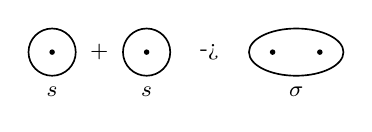
\begin{tikzpicture}
                \footnotesize
                \draw [semithick]
                    (0,0) circle (3mm)
                    (1.2,0) circle (3mm)
                    (3.1,0) ellipse (6mm and 3mm)
                ;

                \fill
                    (0,0) circle (1pt)
                    (1.2,0) circle (1pt)
                    (2.8,0) circle (1pt)
                    (3.4,0) circle (1pt)
                ;
                \node at (0.6,0) {$+$};
                \node at (2,0) {\ce{->}};

                \node at (0,-0.5) {$s$};
                \node at (1.2,-0.5) {$s$};
                \node at (3.1,-0.5) {$\sigma$};
            \end{tikzpicture}
            \caption{Sigma ($\sigma$) bond.}
            \label{fig:sigmaPiDeltaa}
        \end{subfigure}
        \begin{subfigure}[b]{0.3\linewidth}
            \centering
            \begin{tikzpicture}
                \footnotesize
                \filldraw [semithick,fill=grz]
                    (0,0.3) ellipse (3mm and 2mm)
                    (1.2,0.3) ellipse (3mm and 2mm)
                ;
                \draw [semithick]
                    (0,-0.3) ellipse (3mm and 2mm)
                    (1.2,-0.3) ellipse (3mm and 2mm)
                ;
                \draw [semithick,fill=grz] (2.6,0.05)
                    to[out=0,in=180,out looseness=0.5] (3.1,0.12)
                    to[out=0,in=180,in looseness=0.5] (3.6,0.05)
                    to[out=0,in=-90] (3.7,0.15)
                    to[out=90,in=0,out looseness=0.7,in looseness=0.8] (3.1,0.43)
                    to[out=180,in=90,out looseness=0.8,in looseness=0.7] (2.5,0.15)
                    to[out=-90,in=180] cycle
                ;
                \begin{scope}[yscale=-1]
                    \draw [semithick] (2.6,0.05)
                        to[out=0,in=180,out looseness=0.5] (3.1,0.12)
                        to[out=0,in=180,in looseness=0.5] (3.6,0.05)
                        to[out=0,in=-90] (3.7,0.15)
                        to[out=90,in=0,out looseness=0.7,in looseness=0.8] (3.1,0.43)
                        to[out=180,in=90,out looseness=0.8,in looseness=0.7] (2.5,0.15)
                        to[out=-90,in=180] cycle
                    ;
                \end{scope}

                \fill
                    (0,0) circle (1pt)
                    (1.2,0) circle (1pt)
                    (2.8,0) circle (1pt)
                    (3.4,0) circle (1pt)
                ;
                \node at (0.6,0) {$+$};
                \node at (2,0) {\ce{->}};

                \node at (0,-0.7) {$p$};
                \node at (1.2,-0.7) {$p$};
                \node at (3.1,-0.7) {$\pi$};
            \end{tikzpicture}
            \caption{Pi ($\pi$) bond.}
            \label{fig:sigmaPiDeltab}
        \end{subfigure}
        \begin{subfigure}[b]{0.3\linewidth}
            \centering
            \begin{tikzpicture}
                \footnotesize
                \draw [semithick]
                    (0.08,0.01) ellipse (3mm and 2mm)
                    (1.28,0.01) ellipse (3mm and 2mm)
                ;
                \filldraw [semithick,fill=grz]
                    (0,0.3) ellipse (3mm and 2mm)
                    (1.2,0.3) ellipse (3mm and 2mm)
                    (0,-0.3) ellipse (3mm and 2mm)
                    (1.2,-0.3) ellipse (3mm and 2mm)
                ;
                \filldraw [semithick,fill=white]
                    (-0.08,-0.01) ellipse (3mm and 2mm)
                    (1.12,-0.01) ellipse (3mm and 2mm)
                ;
                \draw [semithick]
                    (3.18,0.01) ellipse (6mm and 2mm)
                ;
                \draw [semithick,fill=grz] (2.6,0.05)
                    to[out=0,in=180,out looseness=0.5] (3.1,0.12)
                    to[out=0,in=180,in looseness=0.5] (3.6,0.05)
                    to[out=0,in=-90] (3.7,0.15)
                    to[out=90,in=0,out looseness=0.7,in looseness=0.8] (3.1,0.43)
                    to[out=180,in=90,out looseness=0.8,in looseness=0.7] (2.5,0.15)
                    to[out=-90,in=180] cycle
                ;
                \begin{scope}[yscale=-1]
                    \draw [semithick,fill=grz] (2.6,0.05)
                        to[out=0,in=180,out looseness=0.5] (3.1,0.12)
                        to[out=0,in=180,in looseness=0.5] (3.6,0.05)
                        to[out=0,in=-90] (3.7,0.15)
                        to[out=90,in=0,out looseness=0.7,in looseness=0.8] (3.1,0.43)
                        to[out=180,in=90,out looseness=0.8,in looseness=0.7] (2.5,0.15)
                        to[out=-90,in=180] cycle
                    ;
                \end{scope}
                \filldraw [semithick,fill=white]
                    (3.02,-0.01) ellipse (6mm and 2mm)
                ;

                \fill
                    (0,0) circle (1pt)
                    (1.2,0) circle (1pt)
                    (2.8,0) circle (1pt)
                    (3.4,0) circle (1pt)
                ;
                \node at (0.6,0) {$+$};
                \node at (2,0) {\ce{->}};

                \node at (0,-0.7) {$d$};
                \node at (1.2,-0.7) {$d$};
                \node at (3.1,-0.7) {$\delta$};
            \end{tikzpicture}
            \caption{Delta ($\delta$) bond.}
            \label{fig:sigmaPiDeltac}
        \end{subfigure}
        \caption{Examples of bonding interactions.}
        \label{fig:sigmaPiDelta}
    \end{figure}
    \begin{itemize}
        \item No such bonds exist between carbon atoms because two carbon atoms max out at a triple bond.
        \item Quadruple bonds possess one sigma bond, two pi bonds, and one delta ($\delta$) bond.
        \item The delta bond is only possible with metal atoms because these atoms possess energetically accessible $d$ orbitals.
    \end{itemize}
    \item Quintuple bonds between transition metals have been reported, but scientists have not yet reached a consensus on to what extent these exist.
    \item Hydrogen atoms and alkyl groups can act as bridges in inorganic chemistry, excessively disobeying the octet rule (see Figure \ref{fig:bridgingH-CH3}).
    \begin{figure}[h!]
        \centering
        \footnotesize
        \chemfig{H<:[:-25]B(<[:-155]H)(-[7]H?)-[1]H-[7]B?(>:[:25]H)<[:-25]H}
        \hspace{5em}
        \chemfig{H_3C<:[:-25]Al(<[:-155]H_3C)(-[7]\chembelow{C}{\hspace{4pt}H_3}?)-[1]\chemabove{C}{\hspace{4pt}H_3}-[7]Al?(>:[:25]CH_3)<[:-25]CH_3}
        \caption{Inorganic compounds containing bridging hydrogens and alkyl groups.}
        \label{fig:bridgingH-CH3}
    \end{figure}
    \item \textbf{Coordination number}: The number of other atoms, molecules, or ions to which an atom is bonded.
    \item "Numerous inorganic compounds have central atoms with coordination numbers of five, six, seven, and higher" \parencite[2]{bib:MiesslerFischerTarr}.
    \begin{itemize}
        \item The most common coordination geometry for transition metals is octahedral.
    \end{itemize}
    \item 4-coordinate carbon is almost always tetrahedral. 4-coordinate metals and nonmetals can be either tetrahedral or square planar.
    \item \textbf{Coordination complex}: A compound with a metal as the central atom or ion and some number of \textbf{ligands} bonded to it.
    \item \textbf{Ligand}: An anion or neutral molecule bonded to a central atom (frequently through \ce{N}, \ce{O}, or \ce{S}).
    \item \textbf{Organometallic complex}: A coordination complex where carbon (potentially bonded to other things) is one of the ligands.
    \item There are multiple kinds of tetrahedral structures. There is the standard arrangement seen in molecules such as methane, but there is also a form that lacks a central atom, as in elemental phosphorous \ce{P4} (see Figure \ref{fig:tetrahedralNoCentral}).
    \begin{figure}[h!]
        \centering
        \footnotesize
        \chemfig[atom sep=5em]{P?[1]-[:53]P(-[6]P?[1]?[3])-[:-53]P?[3]?[1,1,{dash pattern=on 2pt off 2pt}]}
        \caption{Tetrahedral geometry without a central atom.}
        \label{fig:tetrahedralNoCentral}
    \end{figure}
    \begin{itemize}
        \item Other atoms such as boron and carbon also form units that surround a central cavity (e.g., icosahedral \ce{B12} and buckyballs \ce{C60}).
    \end{itemize}
    \item Aromatic rings can bond to metals using all of their pi orbitals. This results in a metal suspended above the ring's center.
    \item \textbf{Cluster compound}: A compound where "a carbon atom is at the center of a polyhedron of metal atoms" \parencite[3]{bib:MiesslerFischerTarr}.
    \begin{itemize}
        \item There exist examples of carbon surrounded by five, six, or more metal atoms\footnote{This provides a challenge to theoretical inorganic chemists.}.
    \end{itemize}
    \item Many new forms of elemental carbon have been discovered since the mid-1980s, notably including fullerenes (such as buckminsterfullerene, or buckyballs), carbon nanotubes, graphene, and polyyne wires.
    \item \textcite{bib:MiesslerFischerTarr} give a brief history of inorganic chemistry for context.
    \begin{itemize}
        \item Be aware of \textbf{crystal field theory} and \textbf{ligand field theory}.
    \end{itemize}
\end{itemize}
\newpage



\section{Chapter 2: Atomic Structure}
\emph{From \textcite{bib:MiesslerFischerTarr}.}
\begin{itemize}
    \item \marginnote{12/22:}\textbf{Coinage metals}: Copper, silver, and gold, i.e., the transition metals in IUPAC Group 11.
    \item \textbf{Chalcogens}: Oxygen, sulfur, selenium, tellurium, and polonium, i.e., the nonmetals in Group 16.
    \item The energies of visible light emitted by the hydrogen atom are given by\footnote{Refer to \textcite{bib:APChemNotes}, specifically Figure 7.6 and the accompanying discussion.}
    \begin{equation*}
        E = R_H\left( \frac{1}{2^2}-\frac{1}{n_h^2} \right)
    \end{equation*}
    where $n_h$ is an integer greater than 2 and $R_H$ is the Rydberg constant for hydrogen (\ce{H}).
    \begin{itemize}
        \item Note that $
            R_H = \SI{1.097e7}{\per\meter}
            = \SI{2.179e-18}{\joule}
            = \SI{13.61}{eV}
        $.
        \item This equation was first discovered by Johann Balmer in 1885.
        \item Infrared and ultraviolet emissions can be described by replacing $2^2$ with integers $n_l^2$ in the above equation on the condition that $n_l<n_h$\footnote{$n_l$ denotes the \underline{l}ower final energy level while $n_h$ denotes the \underline{h}igher initial energy level.}.
    \end{itemize}
    \item The energy of the light emitted is related to its wavelength, frequency, and wavenumber by the equations
    \begin{equation*}
        E = h\nu = \frac{hc}{\lambda} = hc\bar{\nu}
    \end{equation*}
    where $h$ is Planck's constant ($\SI{6.626e-34}{\joule\second}$), $c$ is the speed of light ($\SI{2.998e8}{\meter\per\second}$), $\nu$ is the frequency of the light, $\lambda$ is the wavelength of the light, and $\bar{\nu}$ is the \textbf{wavenumber} of the light.
    \item \textbf{Wavenumber}: The number of waves that exist between two points along the light's path a given distance apart. \emph{Units} waves per centimeter (SI: $\si{\per\centi\meter}$).
    \begin{itemize}
        \item Wavenumber is directly proportional to energy. This is why $\si{\per\meter}$ or $\si{\per\centi\meter}$ can be used as an energy unit.
    \end{itemize}
    \item \textbf{Principal quantum number}: One of the quantities $n$ in Balmer's equation.
    \item Bohr's atomic theory first explained the phenomenon of Balmer's equation, positing that "electrons may absorb light of certain specific energies and be excited to orbits of higher energy; they may also emit light of specific energies and fall to orbits of lower energy" \parencite[11-12]{bib:MiesslerFischerTarr}.
    \begin{itemize}
        \item Bohr rewrote the Rydberg constant in terms of other quantities:
        \begin{equation*}
            R = \frac{2\pi^2\mu Z^2e^4}{(4\pi\varepsilon_0)^2h^2}
        \end{equation*}
        where\dots
        \begin{itemize}
            \item $\mu$ is the reduced mass of the electron/nucleus combination $\frac{1}{\mu}=\frac{1}{m_e}+\frac{1}{m_\text{nucleus}}$, where $m_e=\SI{9.11e-31}{\kilo\gram}$ is the mass of the electron and $m_\text{nucleus}$ is the mass of the nucleus.
            \item $Z$ is the nuclear charge.
            \item $e=\SI{1.602e-19}{\coulomb}$ is the charge of the electron.
            \item $h=\SI{6.626e-34}{\joule\second}$ is Planck's constant.
            \item $\varepsilon_0=\SI{8.85e-12}{\newton\meter\squared\per\coulomb\squared}$ is the permittivity of a vacuum.
        \end{itemize}
        \item Importantly, note that the Rydberg constant for hydrogen $R_H$ is not universal, and changes for the atom at hand based on factors like the mass of the nucleus.
        \item Also note that some of the terms cancel or can be written in terms of others, making the above equation equivalent to the one given in Chapter 7 of \textcite{bib:APChemNotes}.
    \end{itemize}
    \begin{figure}[h!]
        \centering
        \begin{tikzpicture}[yscale=17]
            \footnotesize
            \foreach \y in {1,...,6} {
                \draw [thick] (0,{-1/(\y*\y)}) -- ++(10.5,0) node[right]{$\y$};
            }
            \foreach \y in {7,...,11} {
                \draw [thick] (0,{-1/(\y*\y)}) -- ++(10.5,0);
            }
            \fill (0,{-1/121}) rectangle (10.5,0) node[right]{$\infty$};
    
            \foreach \x in {1,...,5} {
                \draw [semithick,grx,-latex] ({0.05+\x*0.25},{-1/(\x+1)^2}) -- ({0.05+\x*0.25},-1);
            }
            \node [anchor=west,text width=1cm,align=center] at (1.4,{(-1/1-1/4)/2}) {Lyman series (UV)};
            \foreach \x in {2,...,5} {
                \draw [semithick,grx,-latex] ({3.05+\x*0.25},{-1/(\x+1)^2}) -- ({3.05+\x*0.25},{-1/4});
            }
            \node [anchor=west,text width=4cm] at (4.4,{(-1/4-1/9)/2}) {Balmer series\\ (visible transitions shown)};
            \foreach \x in {3,...,5} {
                \draw [semithick,grx,-latex] ({6.05+\x*0.25},{-1/(\x+1)^2}) -- ({6.05+\x*0.25},{-1/9});
            }
            \node [anchor=west] at (7.4,{(-1/9-1/16)/2}) {Paschen series (IR)};
        \end{tikzpicture}
        \caption{Hydrogen atom energy levels.}
        \label{fig:energyLevelH}
    \end{figure}
    \item \textbf{Balmer series}: The four main electron transitions in hydrogen that release electromagnetic radiation in the visible spectrum.
    \item \textbf{Lyman series}: The five main electron transitions in hydrogen that release electromagnetic radiation in the ultraviolet spectrum.
    \item \textbf{Paschen series}: The three main electron transitions in hydrogen that release electromagnetic radiation in the infrared spectrum.
    \item "The inverse square dependence of energy on $n$ results in energy levels that are far apart in energy at small $n$ and become much closer in energy at larger $n$" \parencite[12]{bib:MiesslerFischerTarr}
    \begin{itemize}
        \item Individual electrons can have more energy than they would possess in the infinite energy level, but at and above this point, the nucleus and electron are considered to be separate entities.
    \end{itemize}
    \item \textbf{Heisenberg's uncertainty principle}: "There is a relationship between the inherent uncertainties in the location and momentum of an electron" \parencite[14]{bib:MiesslerFischerTarr}.
    \begin{equation*}
        \Delta x\, \Delta p_x \geq \frac{h}{4\pi}
    \end{equation*}
    \begin{itemize}
        \item The above equation describes the $x$-component of the uncertainty, where $\Delta x$ is the uncertainty in the position of the electron and $\Delta p_x$ is the uncertainty in the momentum of the electron in the $x$-direction.
    \end{itemize}
    \item Because of the uncertainty principle, we cannot treat electrons as particles with precisely described motion; instead, we must describe them in \textbf{orbitals}.
    \item \textbf{Orbital}: A region that describes the probable locations of an electron.
    \item \textbf{Electron density}: "The probability of finding the electron at a particular point in space" \parencite[14]{bib:MiesslerFischerTarr}.
    \begin{itemize}
        \item This can be calculated in principle.
    \end{itemize}
    \item Schr\"{o}dinger and Heisenberg published (in 1926 and 1927, respectively) papers on atomic wave mechanics. Although they used very different mathematical techniques, their theories can be shown to be equivalent. However, we will introduce Schr\"{o}dinger's more commonly used differential equations.
    \item "The Schr\"{o}dinger equation describes the wave properties of an electron in terms of its position, mass, total energy, and potential energy" \parencite[14]{bib:MiesslerFischerTarr}.
    \begin{equation*}
        H\Psi = E\Psi
    \end{equation*}
    \begin{itemize}
        \item In its simplest form, it is given by the above, where $H$ is the \textbf{Hamiltonian operator}, $E$ is the energy of the electron, and $\Psi$ is the \textbf{wave function} of the electron.
    \end{itemize}
    \item \textbf{Wave function}: A function that describes an electron wave in space, i.e., an atomic orbital.
    \item Energy values are another way of describing the quantization introduced with the Bohr model; different orbitals, characterized by different wave functions, each have characteristic energies.
    \item \textbf{Operator}: "An instruction or set of instructions that states what to do with the function that follows it" \parencite[14]{bib:MiesslerFischerTarr}.
    \item \textbf{Hamiltonian operator}: An operator including derivatives that transforms the wave function $\Psi$ into a constant (the energy) times itself ($E\Psi$). \emph{Denoted by} $\bm{H}$, $\bm{\hat{H}}$.
    \begin{equation*}
        H = \frac{-h^2}{8\pi^2m}\left( \pdv[2]{x}+\pdv[2]{y}+\pdv[2]{z} \right)-\frac{Ze^2}{4\pi\varepsilon_0\sqrt{x^2+y^2+z^2}}
    \end{equation*}
    \begin{itemize}
        \item In the form used for calculating the energy levels of one-electron systems, it is given by the above, where\dots
        \begin{itemize}
            \item $h,Z,e,\varepsilon_0$ are defined as in Bohr's definition of the Rydberg constant, above.
            \item $m=m_e$ is the mass of the electron, as defined above.
            \item $\sqrt{x^2+y^2+z^2}=r$ is the distance from the nucleus.
        \end{itemize}
        \item The first part describes the kinetic energy of the electron, i.e., its energy of motion.
        \item The second part describes the potential energy of the electron, the result of the electrostatic attraction between it and the nucleus. It is commonly denoted by $V(x,y,z)$.
    \end{itemize}
    \item "Because $n$ varies from 1 to $\infty$, and every atomic orbital is described by a unique $\Psi$, there is no limit to the number of solutions of the Schr\"{o}dinger equation for an atom. Each $\Psi$ describes the wave properties of a given electron in a particular orbital" \parencite[15]{bib:MiesslerFischerTarr}.
    \item Electron density is proportional to $\Psi^2$.
    \item Necessary conditions for a physically realistic solution for $\Psi$:
    \begin{enumerate}
        \item $\Psi$ must be single-valued: There cannot be two probabilities for an electron at any position in space.
        \item $\Psi$ and its first derivatives must be continuous: The probability must be defined at all positions in space and cannot change abruptly from one point to the next.
        \item $\Psi$ must approach zero as $r\to\infty$: For large distances from the nucleus, the probability must grow smaller and smaller (the atom must be finite).
        \item The integral
        \begin{equation*}
            \int\limits_\text{all space}\Psi_A\Psi_A^*\dd{\tau} = 1
        \end{equation*}
        The total probability of an electron being somewhere in space must be 1. Applying this stipulation is called \textbf{normalizing} the wave function\footnote{$\Psi_A^*$ denotes the complex conjugate of $\Psi_A$. This is necessary because wave functions may have imaginary values. However, in many cases, the wave functions are real and the integrand reduces to $\Psi_A^2$.}.
        \item The integral
        \begin{equation*}
            \int\limits_\text{all space}\Psi_A\Psi_B^*\dd{\tau} = 0
        \end{equation*}
        $\Psi_A$ and $\Psi_B$ are different orbitals within the same atom, and this stipulation reflects the fact that all orbitals in the same atom must be \textbf{orthogonal} to each other.
    \end{enumerate}
    \item \marginnote{12/23:}The Particle in a Box.
    \begin{itemize}
        \item Imagine a one-dimensional "box" between $x=0$ and $x=a$ with potential energy everywhere zero inside the "box" and everywhere infinite outside the box.
        \begin{itemize}
            \item These energy constraints mean that the particle is completely trapped within the box (it would take an infinite amount of energy to leave), but also that no forces act on it within the box.
        \end{itemize}
        \item It follows that the wave equation for locations within the box is
        \begin{equation*}
            \frac{-h^2}{8\pi^2m}\left( \pdv[2]{\Psi(x)}{x} \right) = E\Psi(x)
        \end{equation*}
        \item Since sine and cosine functions have properties associated with waves, we propose that a general solution describing possible waves in the box is
        \begin{equation*}
            \Psi(x) = A\sin rx+B\cos sx
        \end{equation*}
        where $A,B,r,s$ are constants\footnote{It can be proven mathematically that this "ansatz" \emph{is} the (real) general solution to the given differential equation. See \textcite{bib:MATH27300Notes}.}.
        \item As seen in Problem 2.8a, substituting the above general solution into the wave equation allows us to solve for
        \begin{equation*}
            r = s = \sqrt{2mE}\cdot\frac{2\pi}{h}
        \end{equation*}
        \item Because $\Psi$ must be continuous and equal 0 for $x<0$ and $x>a$, $\Psi$ must approach 0 as $x\to 0$ and $x\to a$. Since $\cos(s\cdot 0)=1$, $\Psi(0)$ can only equal 0 if $B=0$. Therefore, the wave function reduces to
        \begin{equation*}
            \Psi(x) = A\sin rx
        \end{equation*}
        \item We must also have $\Psi(a)=0$, which is only possible if $rx$ is an integer multiple of $\pi$. This means that
        \begin{align*}
            ra &= \pm n\pi\\
            r &= \frac{\pm n\pi}{a}
        \end{align*}
        \item Combining the two expressions for $r$, we can solve for $E$:
        \begin{equation*}
            E = \frac{n^2h^2}{8ma^2}
        \end{equation*}
        \begin{itemize}
            \item "These are the energy levels predicted by the particle-in-a-box model for any particle in a one dimensional box of length $a$. The energy levels are quantized according to quantum numbers $n=1,2,3,\dots$" \parencite[17]{bib:MiesslerFischerTarr}.
        \end{itemize}
        \item As seen in Problem 2.8d, substituting $r=n\pi/a$ into $\Psi(x)$ and applying the normalizing requirement allows us to solve for the total solution
        \begin{equation*}
            \Psi(x) = \sqrt{\frac{2}{a}}\sin\frac{n\pi x}{a}
        \end{equation*}
        \item The predicted probability densities for an electron at different energy levels (see Figure \ref{fig:particleInABox}) showcase a difference between classical mechanics' and quantum mechanics' predictions about the behavior of this particle: Classical predicts an equal probability at any point in the box, but the (quantum) wave nature of the particle predicts varied probabilities in different locations.
        \begin{figure}[h!]
            \centering
            \footnotesize
            \begin{subfigure}[b]{0.33\linewidth}
                \centering
                \begin{tikzpicture}[xscale=4,yscale=0.7]
                    \draw (0,-2) -- node[below=6mm]{\small$x/a$} (1,-2);
                    \draw (0,-2) -- (0,2);
                    \foreach \x in {0,0.2,0.4,0.6,0.8,1} {
                        \draw (\x,-2) -- ++(0,-0.2) node[below]{$\x$};
                    }
                    \foreach \y in {-2,...,2} {
                        \draw (0,\y) -- ++(-0.04,0) node[left]{$\y$};
                    }
                    \draw [dashed] (0,0) -- (1,0);
        
                    \draw [grx,thick] plot[domain=0:1,samples=100,smooth] (\x,{2^0.5*sin(pi*\x r)});
                    \draw [gry,thick] plot[domain=0:1,samples=100,smooth] (\x,{(2^0.5*sin(pi*\x r))^2});
                    \node [inner sep=0pt] at (0.8,1.7) {$\Psi^2$}
                        edge (0.67,{(2^0.5*sin(pi*0.67 r))^2})
                    ;
                    \node [inner sep=0pt] at (0.95,1) {$\Psi$}
                        edge (0.84,{2^0.5*sin(pi*0.84 r)})
                    ;
                \end{tikzpicture}
                \caption{$n=1$.}
                \label{fig:particleInABoxa}
            \end{subfigure}
            \begin{subfigure}[b]{0.32\linewidth}
                \centering
                \begin{tikzpicture}[xscale=4,yscale=0.7]
                    \draw (0,-2) -- node[below=6mm]{\small$x/a$} (1,-2);
                    \draw (0,-2) -- (0,2);
                    \foreach \x in {0,0.2,0.4,0.6,0.8,1} {
                        \draw (\x,-2) -- ++(0,-0.2) node[below]{$\x$};
                    }
                    \foreach \y in {-2,...,2} {
                        \draw (0,\y) -- ++(-0.04,0) node[left]{$\y$};
                    }
                    \draw [dashed] (0,0) -- (1,0);
        
                    \draw [grx,thick] plot[domain=0:1,samples=100,smooth] (\x,{2^0.5*sin(2*pi*\x r)});
                    \draw [gry,thick] plot[domain=0:1,samples=100,smooth] (\x,{(2^0.5*sin(2*pi*\x r))^2});
                    \node [inner sep=0pt] at (0.96,1.7) {$\Psi^2$}
                        edge (0.84,{(2^0.5*sin(2*pi*0.84 r))^2})
                    ;
                    \node [inner sep=0pt] at (0.95,-1.5) {$\Psi$}
                        edge (0.84,{2^0.5*sin(2*pi*0.84 r)})
                    ;
                \end{tikzpicture}
                \caption{$n=2$.}
                \label{fig:particleInABoxb}
            \end{subfigure}
            \begin{subfigure}[b]{0.33\linewidth}
                \centering
                \begin{tikzpicture}[xscale=4,yscale=0.7]
                    \draw (0,-2) -- node[below=6mm]{\small$x/a$} (1,-2);
                    \draw (0,-2) -- (0,2);
                    \foreach \x in {0,0.2,0.4,0.6,0.8,1} {
                        \draw (\x,-2) -- ++(0,-0.2) node[below]{$\x$};
                    }
                    \foreach \y in {-2,...,2} {
                        \draw (0,\y) -- ++(-0.04,0) node[left]{$\y$};
                    }
                    \draw [dashed] (0,0) -- (1,0);
        
                    \draw [grx,thick] plot[domain=0:1,samples=100,smooth] (\x,{2^0.5*sin(3*pi*\x r)});
                    \draw [gry,thick] plot[domain=0:1,samples=100,smooth] (\x,{(2^0.5*sin(3*pi*\x r))^2});
                    \node [inner sep=0pt] at (0.67,1.7) {$\Psi^2$}
                        edge (0.78,{(2^0.5*sin(3*pi*0.78 r))^2})
                    ;
                    \node [inner sep=0pt] at (0.7,-1) {$\Psi$}
                        edge (0.6,{2^0.5*sin(3*pi*0.6 r)})
                    ;
                \end{tikzpicture}
                \caption{$n=3$.}
                \label{fig:particleInABoxc}
            \end{subfigure}
            \caption{Particle in a box: Wave functions and their squares at different energy levels.}
            \label{fig:particleInABox}
        \end{figure}
        \begin{itemize}
            \item "The greater the square of the electron amplitude, the greater the probability of the electron being located at the specified coordinate when at the quantized energy defined by $\Psi$" \parencite[17]{bib:MiesslerFischerTarr}.
        \end{itemize}
    \end{itemize}
    \item Atomic orbitals, mathematically, are discrete solutions of the three-dimensional Schr\"{o}dinger equations.
    \begin{itemize}
        \item These orbital equations include four quantum numbers (see Table \ref{tab:quantumNumbers}).
        \item Orbitals with $l$ values $0,1,2,3,4,\dots$ are known by the labels $s,p,d,f,g,\dots$(continuing alphabetically), respectively, derived from early terms for different families of spectroscopic lines.
        \begin{table}[H]
            \centering
            \renewcommand{\arraystretch}{1.4}
            \small
            \begin{tabular}{lllp{4.7cm}}
                \noalign{\global\arrayrulewidth=1pt}\arrayrulecolor{gry}\hline
                \rowcolor{grx}
                \textcolor{white}{\textbf{Symbol}} & \textcolor{white}{\textbf{Name}} & \textcolor{white}{\textbf{Values}} & \textcolor{white}{\textbf{Role}}\\
                $n$ & Principal & $1,2,3,\dots$ & Determines the major part of the energy.\\
                \rowcolor{grt}
                $l$ & Angular momentum\footnotemark & $0,1,2,\dots,n-1$ & Describes angular dependence and contributes to the energy.\\
                $m_l$ & Magnetic & $0,\pm 1,\pm 2,\dots,\pm l$ & Describes orientation in space (angular momentum in the $z$-direction).\\
                \rowcolor{grt}
                $m_s$ & Spin & $\pm\frac{1}{2}$ & Describes orientation of the electron spin (magnetic moment) in space.\\
                \arrayrulecolor{grx}\hline
                \noalign{\global\arrayrulewidth=0.4pt}
            \end{tabular}
            \caption{Quantum numbers and their properties.}
            \label{tab:quantumNumbers}
        \end{table}
        \footnotetext{\emph{Also known as} \textbf{azimuthal} (quantum number).}
        \item $n$ is the primary quantum number affecting the overall energy.
        \item $l$ determines the type of shape. See Table \ref{tab:WaveFunctionsAngular-H}.
        \item $m_l$ determines the "orientation of the angular momentum vector in a magnetic field, or the position of the orbital in space" \parencite[18]{bib:MiesslerFischerTarr}. See Table \ref{tab:WaveFunctionsAngular-H}.
        \item $m_s$ determines the electron spin\footnote{Note that the spin of an electron is purely quantum mechanical, and should not be related back to classical mechanics.} in the orbital, or "the orientation of the electron's magnetic moment in a magnetic field, either in the direction of the field ($+\frac{1}{2}$) or opposed to it ($-\frac{1}{2}$)" \parencite[18]{bib:MiesslerFischerTarr}.
        \item $n$, $l$, and $m_l$ specify an orbital; $m_s$ specifies one of the two electrons in the orbital.
    \end{itemize}
    \item A note on $i=\sqrt{-1}$ in Table \ref{tab:WaveFunctionsAngular-H}:
    \begin{itemize}
        \item Any linear combination of solutions to the wave equation is another solution.
        \item Because it is more convenient to work with real functions as opposed to complex functions, we make use of the above fact to decomplexify the solutions, as in the following examples.
        \begin{align*}
            \Psi_{2p_x} &= \frac{1}{\sqrt{2}}(\Psi_{+1}+\Psi_{-1})\\
            &= \frac{1}{\sqrt{2}}\left( \frac{1}{\sqrt{2\pi}}\e[i\phi]\cdot\frac{\sqrt{3}}{2}\sin\theta\cdot[R(r)]+\frac{1}{\sqrt{2\pi}}\e[-i\phi]\cdot\frac{\sqrt{3}}{2}\sin\theta\cdot[R(r)] \right)\\
            &= \left( \frac{1}{\sqrt{\pi}}\frac{\sqrt{3}}{2}[R(r)]\sin\theta \right)\frac{\e[i\phi]+\e[-i\phi]}{2}\\
            &= \frac{1}{2}\sqrt{\frac{3}{\pi}}[R(r)]\sin\theta\cos\phi
        \end{align*}
        \begin{align*}
            \Psi_{2p_y} &= \frac{-i}{\sqrt{2}}(\Psi_{+1}-\Psi_{-1})\footnotemark\\
            &= \left( \frac{1}{\sqrt{\pi}}\frac{\sqrt{3}}{2}[R(r)]\sin\theta \right)\frac{\e[i\phi]-\e[-i\phi]}{2i}\\
            &= \frac{1}{2}\sqrt{\frac{3}{\pi}}[R(r)]\sin\theta\sin\phi
        \end{align*}
        \footnotetext{Errata: \textcite{bib:MiesslerFischerTarr} incorrectly normalizes this expression with $i/\sqrt{2}$.}
    \end{itemize}
    \pagebreak
    \begin{table}[h!]
        \centering
        \renewcommand{\arraystretch}{1.6}
        \setlength{\tabcolsep}{1mm}
        \small
        \begin{tabular}{llllcllcl}
            \rowcolor{grx}
            \multicolumn{5}{c}{\textcolor{white}{\textbf{Angular factors}}} & \multicolumn{4}{c}{\textcolor{white}{\textbf{Real Wave Functions}}}\\
            \rowcolor{grx}
            \multicolumn{4}{c}{\textcolor{white}{\textbf{Related to Angular Momentum}}} & \begin{tabular}{c}\textcolor{white}{\textbf{Functions}}\\[-5pt]\textcolor{white}{\textbf{of $\bm{\theta}$}}\end{tabular} & \textcolor{white}{\textbf{In Polar Coordinates}} & \begin{tabular}{c}\textcolor{white}{\textbf{In Cartesian}}\\[-5pt]\textcolor{white}{\textbf{Coordinates}}\end{tabular} & \textcolor{white}{\textbf{Shapes}} & \textcolor{white}{\textbf{Label}}\\
            $l$ & $m_l$ & $\Phi$ & $\Theta$ & & $\Theta\Phi(\theta,\phi)$ & $\Theta\Phi(x,y,z)$\\
    
            $0(s)$ & $0$ & $\dfrac{1}{\sqrt{2\pi}}$ & $\dfrac{1}{\sqrt{2}}$ & \tikz[scale=0.4,baseline={(0,0)}]{
                \footnotesize
                \draw (0,0) -- (1.7,0);
                \draw [-latex] (0,-1.7) -- (0,1.7) node[above]{$z$};
                %
                \draw [semithick] plot[domain=-pi/2:pi/2,smooth,variable=\thta] ({\thta r}:{1/2^0.5});
            } & $\dfrac{1}{2\sqrt{\pi}}$ & $\dfrac{1}{2\sqrt{\pi}}$ & \tikz[scale=0.4,baseline={(0,0)}]{
                \draw [white,-latex] (-1.7,0,0) -- (1.7,0,0) node[right=-1pt]{$x$};
                \draw [white,-latex] (0,-1.7,0) -- (0,1.7,0) node[above right=-2pt]{$z$};
                \draw [semithick] plot[domain=0:2*pi,smooth,variable=\thta] ({\thta r}:1);
            } & $s$\\
    
            $1(p)$ & $0$ & $\dfrac{1}{\sqrt{2\pi}}$ & $\dfrac{\sqrt{6}}{2}\cos\theta$ & \tikz[scale=0.4,baseline={(0,0)}]{
                \footnotesize
                \draw [white,-latex] (0,-1.7) -- (0,1.7) node{$z$};
                \draw (0,0) -- (1.7,0);
                \draw (0,-1.7) -- (0,1.7);
                %
                \draw [semithick] plot [domain=0:pi/2,smooth,variable=\thta] ({\thta r}:{6^0.5/2*sin(\thta r)});
                \draw [semithick] plot [domain=pi/2:pi,smooth,variable=\thta] ({\thta r}:{-6^0.5/2*sin(\thta r)});
            } & $\dfrac{1}{2}\sqrt{\dfrac{3}{\pi}}\cos\theta$ & $\dfrac{1}{2}\sqrt{\dfrac{3}{\pi}}\dfrac{z}{r}$ & \tikz[scale=0.4,baseline={(0,0)},z={(0.8,0.65)}]{
                \footnotesize
                \draw [-latex] (-1.7,0,0) -- (1.7,0,0) node[right=-1pt]{$x$};
                \draw [-latex] (0,-1.7,0) -- (0,1.7,0) node[above right=-2pt]{$z$};
                \filldraw [semithick,fill=grz] (0,{-6^0.5/4},0) circle (6^0.5/4);
                \draw [-latex] (0,0,-1.7) -- (0,0,1.7) node[above right=-2pt]{$y$};
                \filldraw [semithick,fill=white] (0,{6^0.5/4},0) circle (6^0.5/4);
            } & $p_z$\\
    
            & $+1$ & $\dfrac{1}{\sqrt{2\pi}}\e[i\phi]$ & $\dfrac{\sqrt{3}}{2}\sin\theta$ & \multirow{2}{*}{\tikz[scale=0.4,baseline={(0,0)}]{
                \footnotesize
                \draw [white,-latex] (0,-2.2) -- (0,2.2) node{$z$};
                \draw (0,0) -- (1.7,0);
                \draw (0,-1.7) -- (0,1.7);
                %
                \draw [semithick] plot [domain=0:pi,smooth,variable=\thta] ({\thta r}:{3^0.5/2*cos(\thta r)});
            }} & $\dfrac{1}{2}\sqrt{\dfrac{3}{\pi}}\sin\theta\cos\phi$ & $\dfrac{1}{2}\sqrt{\dfrac{3}{\pi}}\dfrac{x}{r}$ & \tikz[scale=0.4,baseline={(0,0)},z={(0.8,0.65)}]{
                \footnotesize
                \draw [white,-latex] (-1.7,0,0) -- (1.7,0,0) node[right=-1pt]{$x$};
                \draw [white,-latex] (0,-1.7,0) -- (0,1.7,0) node[above right=-2pt]{$z$};
                \draw (-1.7,0,0) -- (1.7,0,0);
                \draw (0,-1.7,0) -- (0,1.7,0);
                \filldraw [semithick,fill=grz] ({-6^0.5/4},0,0) circle (6^0.5/4);
                \draw (0,0,-1.7) -- (0,0,1.7);
                \filldraw [semithick,fill=white] ({6^0.5/4},0,0) circle (6^0.5/4);
            } & $p_x$\\
    
            & $-1$ & $\dfrac{1}{\sqrt{2\pi}}\e[-i\phi]$ & $\dfrac{\sqrt{3}}{2}\sin\theta$ & & $\dfrac{1}{2}\sqrt{\dfrac{3}{\pi}}\sin\theta\sin\phi$ & $\dfrac{1}{2}\sqrt{\dfrac{3}{\pi}}\dfrac{y}{r}$ & \tikz[scale=0.4,baseline={(0,0)},z={(0.8,0.65)}]{
                \footnotesize
                \draw [white,-latex] (-1.7,0,0) -- (1.7,0,0) node[right=-1pt]{$x$};
                \draw [white,-latex] (0,-1.7,0) -- (0,1.7,0) node[above right=-2pt]{$z$};
                \filldraw [semithick,fill=white] (0,0,{6^0.5/4}) circle (6^0.5/4);
                \draw (-1.7,0,0) -- (1.7,0,0);
                \draw (0,-1.7,0) -- (0,1.7,0);
                \filldraw [semithick,fill=grz] (0,0,{-6^0.5/4}) circle (6^0.5/4);
                \draw (0,0,-1.7) -- (0,0,-0.85) (0,0,{6^0.5/2}) -- (0,0,1.7);
            } & $p_y$\\
    
            $2(d)$ & $0$ & $\dfrac{1}{\sqrt{2\pi}}$ & $\dfrac{1}{2}\sqrt{\dfrac{5}{2}}(3\cos^2\theta-1)$ & \tikz[scale=0.4,baseline={(0,0)}]{
                \footnotesize
                \draw [white,-latex] (0,-1.7) -- (0,1.7) node{$z$};
                \draw (0,0) -- (1.7,0);
                \draw (0,-1.7) -- (0,1.7);
                %
                \draw [semithick] plot [domain=0.63:1.57,smooth,variable=\thta] ({\thta r}:{0.5*2.5^0.5*(3*sin(\thta r)^2-1)});
                \draw [semithick] plot [domain=2.53:3.75,smooth,variable=\thta] ({\thta r}:{0.5*2.5^0.5*(3*sin(\thta r)^2-1)});
                \draw [semithick] plot [domain=4.71:5.67,smooth,variable=\thta] ({\thta r}:{0.5*2.5^0.5*(3*sin(\thta r)^2-1)});
            } & $\dfrac{1}{4}\sqrt{\dfrac{5}{\pi}}(3\cos^2\theta-1)$ & $\dfrac{1}{4}\sqrt{\dfrac{5}{\pi}}\dfrac{2z^2-x^2-y^2}{r^2}$ & \tikz[scale=0.4,baseline={(0,0)},z={(0.8,0.65)}]{
                \footnotesize
                \draw [white,-latex] (-1.7,0,0) -- (1.7,0,0) node[right=-1pt]{$x$};
                \draw [white,-latex] (0,-1.7,0) -- (0,1.7,0) node[above right=-2pt]{$z$};
                \draw (-1.7,0,0) -- (1.7,0,0);
                \draw (0,-1.7,0) -- (0,1.7,0);
                \filldraw [semithick,fill=white] plot [domain=0.63:2.51,smooth,variable=\thta] ({\thta r}:{0.5*2.5^0.5*(3*sin(\thta r)^2-1)});
                \filldraw [semithick,fill=white] plot [domain=3.75:5.67,smooth,variable=\thta] ({\thta r}:{0.5*2.5^0.5*(3*sin(\thta r)^2-1)});
                \draw (0,0,-1.7) -- (0,0,1.7);
                \filldraw [semithick,fill=grz] (-0.4,0,0) arc[start angle=120,end angle=60,x radius=0.8cm,y radius=0.9cm] arc[start angle=-60,end angle=-120,x radius=0.8cm,y radius=0.9cm];
                \filldraw [semithick,fill=white] ({0.73 r}:{0.5*2.5^0.5*(3*sin(0.73 r)^2-1)}) to[out=-125,in=-55] ({2.41 r}:{0.5*2.5^0.5*(3*sin(2.41 r)^2-1)});
            } & $d_{z^2}$\\
    
            & $+1$ & $\dfrac{1}{\sqrt{2\pi}}\e[i\phi]$ & $\dfrac{\sqrt{15}}{2}\cos\theta\sin\theta$ & \multirow{2}{*}{\tikz[scale=0.4,baseline={(0,0)}]{
                \footnotesize
                \draw [white,-latex] (0,-2.2) -- (0,2.2) node{$z$};
                \draw (0,0) -- (1.7,0);
                \draw (0,-1.7) -- (0,1.7);
                %
                \draw [semithick] plot [domain=0:pi,smooth,variable=\thta] ({\thta r}:{15^0.5/2*cos(\thta r)*sin(\thta r)});
            }} & $\dfrac{1}{2}\sqrt{\dfrac{15}{\pi}}\cos\theta\sin\theta\cos\phi$ & $\dfrac{1}{2}\sqrt{\dfrac{15}{\pi}}\dfrac{xz}{r^2}$ & \tikz[scale=0.4,baseline={(0,0)},z={(0.8,0.65)}]{
                \footnotesize
                \draw [white,-latex] (-1.7,0,0) -- (1.7,0,0) node[right=-1pt]{$x$};
                \draw [white,-latex] (0,-1.7,0) -- (0,1.7,0) node[above right=-2pt]{$z$};
                \draw (-1.7,0,0) -- (1.7,0,0);
                \draw (0,-1.7,0) -- (0,1.7,0);
                \filldraw [semithick,fill=white,scale=1.5] plot [domain=-pi:-pi/2,smooth,variable=\thta] ({\thta r}:{15^0.5/2*cos(\thta r)*sin(\thta r)});
                \filldraw [semithick,fill=grz,scale=1.5] plot [domain=-pi/2:0,smooth,variable=\thta] ({\thta r}:{15^0.5/2*cos(\thta r)*sin(\thta r)});
                \draw (0,0,-1.7) -- (0,0,1.7);
                \filldraw [semithick,fill=white,scale=1.5] plot [domain=0:pi/2,smooth,variable=\thta] ({\thta r}:{15^0.5/2*cos(\thta r)*sin(\thta r)});
                \filldraw [semithick,fill=grz,scale=1.5] plot [domain=pi/2:pi,smooth,variable=\thta] ({\thta r}:{15^0.5/2*cos(\thta r)*sin(\thta r)});
            } & $d_{xz}$\\
    
            & $-1$ & $\dfrac{1}{\sqrt{2\pi}}\e[-i\phi]$ & $\dfrac{\sqrt{15}}{2}\cos\theta\sin\theta$ & & $\dfrac{1}{2}\sqrt{\dfrac{15}{\pi}}\cos\theta\sin\theta\sin\phi$ & $\dfrac{1}{2}\sqrt{\dfrac{15}{\pi}}\dfrac{yz}{r^2}$ & \tikz[scale=0.4,baseline={(0,0)},z={(0.8,0.65)}]{
                \footnotesize
                \draw [white,-latex] (-1.7,0,0) -- (1.7,0,0) node[right=-1pt]{$x$};
                \draw [white,-latex] (0,-1.7,0) -- (0,1.7,0) node[above right=-2pt]{$z$};
                \filldraw [semithick,fill=grz,rotate=25,xscale=1.2,yscale=1.3] plot [domain=pi/2:pi,smooth,variable=\thta] ({\thta r}:{15^0.5/2*cos(\thta r)*sin(\thta r)});
                \filldraw [semithick,fill=white,rotate=25,scale=1.5] plot [domain=0:pi/2,smooth,variable=\thta] ({\thta r}:{15^0.5/2*cos(\thta r)*sin(\thta r)});
                \draw (-1.7,0,0) -- (1.7,0,0);
                \draw (0,-1.7,0) -- (0,1.7,0);
                \filldraw [semithick,fill=white,rotate=25,scale=1.5] plot [domain=-pi:-pi/2,smooth,variable=\thta] ({\thta r}:{15^0.5/2*cos(\thta r)*sin(\thta r)});
                \draw (0,0,-1.7) -- (0,0,1.7);
                \filldraw [semithick,fill=grz,rotate=25,xscale=1.2,yscale=1.3] plot [domain=-pi/2:0,smooth,variable=\thta] ({\thta r}:{15^0.5/2*cos(\thta r)*sin(\thta r)});
            } & $d_{yz}$\\
    
            & $+2$ & $\dfrac{1}{\sqrt{2\pi}}\e[2i\phi]$ & $\dfrac{\sqrt{15}}{4}\sin^2\theta$ & \multirow{2}{*}{\tikz[scale=0.4,baseline={(0,0)}]{
                \footnotesize
                \draw [white,-latex] (0,-2.2) -- (0,2.2) node{$z$};
                \draw (0,0) -- (1.7,0);
                \draw (0,-1.7) -- (0,1.7);
                %
                \draw [semithick] plot [domain=-pi/2:pi/2,smooth,variable=\thta] ({\thta r}:{15^0.5/4*cos(\thta r)^2});
            }} & $\dfrac{1}{4}\sqrt{\dfrac{15}{\pi}}\sin^2\theta\cos 2\phi$ & $\dfrac{1}{4}\sqrt{\dfrac{15}{\pi}}\dfrac{x^2-y^2}{r^2}$ & \tikz[scale=0.4,baseline={(0,0)},z={(0.8,0.65)}]{
                \footnotesize
                \draw [white,-latex] (-1.7,0,0) -- (1.7,0,0) node[right=-1pt]{$x$};
                \draw [white,-latex] (0,-1.7,0) -- (0,1.7,0) node[above right=-2pt]{$z$};
                \filldraw [semithick,fill=grz,scale=1.3,rotate=40] plot [domain=-pi/2:pi/2,smooth,variable=\thta] ({\thta r}:{15^0.5/4*cos(\thta r)^2});
                \draw (-1.7,0,0) -- (1.7,0,0);
                \draw (0,-1.7,0) -- (0,1.7,0);
                \filldraw [semithick,fill=white,scale=1.5] plot [domain=pi/2:3*pi/2,smooth,variable=\thta] ({\thta r}:{15^0.5/4*cos(\thta r)^2});
                \filldraw [semithick,fill=white,scale=1.5] plot [domain=-pi/2:pi/2,smooth,variable=\thta] ({\thta r}:{15^0.5/4*cos(\thta r)^2});
                \filldraw [semithick,fill=grz,scale=1.3,rotate=40] plot [domain=pi/2:3*pi/2,smooth,variable=\thta] ({\thta r}:{15^0.5/4*cos(\thta r)^2});
                \draw (0,0,-1.7) -- (0,0,-1) (0,0,1.2) -- (0,0,1.7);
            } & $d_{x^2-y^2}$\\
    
            & $-2$ & $\dfrac{1}{\sqrt{2\pi}}\e[-2i\phi]$ & $\dfrac{\sqrt{15}}{4}\sin^2\theta$ & & $\dfrac{1}{4}\sqrt{\dfrac{15}{\pi}}\sin^2\theta\sin 2\phi$ & $\dfrac{1}{4}\sqrt{\dfrac{15}{\pi}}\dfrac{xy}{r^2}$ & \tikz[scale=0.4,baseline={(0,0)},z={(0.8,0.65)}]{
                \footnotesize
                \draw [white,-latex] (-1.7,0,0) -- (1.7,0,0) node[right=-1pt]{$x$};
                \draw [white,-latex] (0,-2.5,0) -- (0,1.7,0) node[above right=-2pt]{$z$};
                \filldraw [semithick,fill=grz,scale=1.2,rotate=-60] plot [domain=pi/2:3*pi/2,smooth,variable=\thta] ({\thta r}:{15^0.5/4*cos(\thta r)^2});
                \draw (-1.7,0,0) -- (1.7,0,0);
                \draw (0,-1.7,0) -- (0,1.7,0);
                \filldraw [semithick,fill=white,scale=1.5,rotate=20] plot [domain=pi/2:3*pi/2,smooth,variable=\thta] ({\thta r}:{15^0.5/4*cos(\thta r)^2});
                \draw (0,0,-1.7) -- (0,0,1.7);
                \filldraw [semithick,fill=white,scale=1.5,rotate=20] plot [domain=-pi/2:pi/2,smooth,variable=\thta] ({\thta r}:{15^0.5/4*cos(\thta r)^2});
                \filldraw [semithick,fill=grz,scale=1.4,rotate=-60] plot [domain=-pi/2:pi/2,smooth,variable=\thta] ({\thta r}:{15^0.5/4*cos(\thta r)^2});
            } & $d_{xy}$\\
            \noalign{\global\arrayrulewidth=1pt}\arrayrulecolor{grx}\hline
            \noalign{\global\arrayrulewidth=0.4pt}
        \end{tabular}
        \begin{tikzpicture}[remember picture,overlay]
            \draw [very thick,decorate,decoration=brace,xshift=-0.4cm,yshift=0.6cm] (0,0) -- (0,2.7);
            \draw [very thick,decorate,decoration=brace,xshift=-0.4cm,yshift=3.8cm] (0,0) -- (0,2.7);
            \draw [very thick,decorate,decoration=brace,xshift=-0.4cm,yshift=8.7cm] (0,0) -- (0,2.7);
    
            \draw [very thick,decorate,decoration=brace,xshift=-2.3cm,yshift=0.6cm] (0,2.7) -- (0,0);
            \draw [very thick,decorate,decoration=brace,xshift=-2.3cm,yshift=3.8cm] (0,2.7) -- (0,0);
            \draw [very thick,decorate,decoration=brace,xshift=-2.3cm,yshift=8.7cm] (0,2.7) -- (0,0);
        \end{tikzpicture}
        \caption{Hydrogen atom wave functions: Angular functions.}
        \label{tab:WaveFunctionsAngular-H}
    \end{table}
    \begin{table}[h!]\marginnote{12/23:}
        \centering
        \renewcommand{\arraystretch}{1.6}
        \setlength{\tabcolsep}{5mm}
        \small
        \begin{tabular}{cccl}
            \rowcolor{grx}
            \multicolumn{4}{c}{\textcolor{white}{\textbf{Radial Functions $\bm{R(r)}$, with $\bm{\sigma=Zr/a_0}$}}}\\
            \rowcolor{grx}
            \textcolor{white}{\textbf{Orbital}} & \textcolor{white}{\quad$\bm{n}$\quad} & \textcolor{white}{\quad$\bm{l}$\quad} & \multicolumn{1}{c}{\textcolor{white}{$\bm{R(r)}$}}\\
            
            $1s$ & $1$ & $0$ & $R_{1s}=2\left[ \dfrac{Z}{a_0} \right]^{3/2}\e[-\sigma]$\rule{0pt}{7mm}\\[3.5mm]
            \rowcolor{grt}
            $2s$ & $2$ & $0$ & $R_{2s}=\left[ \dfrac{Z}{2a_0} \right]^{3/2}(2-\sigma)\e[-\sigma/2]$\footnotemark\rule{0pt}{7mm}\\[3.5mm]
            $2p$ &     & $1$ & $R_{2p}=\dfrac{1}{\sqrt{3}}\left[ \dfrac{Z}{2a_0} \right]^{3/2}\sigma\e[-\sigma/2]$\rule{0pt}{7mm}\\[3.5mm]
            \rowcolor{grt}
            $3s$ & $3$ & $0$ & $R_{3s}=\dfrac{2}{27}\left[ \dfrac{Z}{3a_0} \right]^{3/2}(27-18\sigma+2\sigma^2)\e[-\sigma/3]$\rule{0pt}{7mm}\\[3.5mm]
            $3p$ &     & $1$ & $R_{3p}=\dfrac{1}{81\sqrt{3}}\left[ \dfrac{2Z}{a_0} \right]^{3/2}(6-\sigma)\sigma\e[-\sigma/3]$\rule{0pt}{7mm}\\[3.5mm]
            \rowcolor{grt}
            $3d$ &     & $2$ & $R_{3d}=\dfrac{1}{81\sqrt{15}}\left[ \dfrac{2Z}{a_0} \right]^{3/2}\sigma^2\e[-\sigma/3]$\rule{0pt}{7mm}\\[3.5mm]
            
            \noalign{\global\arrayrulewidth=1pt}\arrayrulecolor{grx}\hline
            \noalign{\global\arrayrulewidth=0.4pt}
        \end{tabular}
        \caption{Hydrogen atom wave functions: Radial functions.}
        \label{tab:WaveFunctionsRadial-H}
    \end{table}
    \item Note that $d_{z^2}$ actually uses the function $2z^2-x^2-y^2$, so we should write $d_{2z^2-x^2-y^2}$ but we shorthand for convenience.
    \item Since the functions in the polar and Cartesian coordinates columns of Table \ref{tab:WaveFunctionsAngular-H} are real, $\Psi=\Psi^*$ and $\Psi\Psi^*=\Psi^2$.
    \item \marginnote{12/25:}$\Psi$ may be expressed in terms of Cartesian coordinates $(x,y,z)$ or in terms of spherical coordinates $(r,\theta,\phi)$.
    \begin{figure}[h!]\marginnote{12/25:}
        \centering
        \begin{tikzpicture}[x={(-0.27cm,-0.47cm)},y={(1cm,0cm)},z={(0cm,1cm)}]
            \footnotesize
            \draw (0,0,0) -- (2.5,0,0) node[below left]{$x$};
            \draw (0,0,0) -- (0,2.5,0) node[right]{$y$};
            \draw (0,0,0) -- (0,0,4) node[above]{$z$};
    
            \fill (xyz spherical cs:radius=4,latitude=60,longitude=50) circle (2pt);
            \draw [semithick] (0,0,0) -- node[below,xshift=1mm]{$r$} (xyz spherical cs:radius=4,latitude=60,longitude=50) -- (xyz spherical cs:radius=2,longitude=50) -- cycle;
            \draw [grx,semithick] plot[domain=50:90,smooth,variable=\phii] (xyz spherical cs:radius=1,longitude=\phii);
            \node [below=-2pt] at (xyz spherical cs:radius=1,longitude=70) {$\phi$};
            \draw [grx,semithick] plot[domain=60:90,smooth,variable=\thta] (xyz spherical cs:radius=1,latitude=\thta,longitude=50);
            \node [above=1pt] at (xyz spherical cs:radius=1,latitude=70,longitude=50) {$\theta$};
        \end{tikzpicture}
        \caption{Spherical coordinates.}
        \label{fig:sphericalCoords}
    \end{figure}
    \begin{itemize}
        \item Using spherical coordinates comes with the advantage that $r$ is the distance from the nucleus (see Figure \ref{fig:sphericalCoords}).
        \pagebreak
        \footnotetext{Errata: This differs from the corresponding equation in \textcite{bib:MiesslerFischerTarr} because the textbook is wrong.}
        \item Know the following volume element conversions\footnote{Refer to \textcite{bib:CAAGThomasNotes}, specifically Figure 16.9 and the accompanying discussion.}.
        \begin{equation*}
            \dd{V} = \dd{x}\dd{y}\dd{z}
            = r^2\sin\theta\dd{\theta}\dd{\phi}\dd{r}
        \end{equation*}
        \item The volume of the thin shell between $r$ and $r+\dd{r}$ is as follows, and is useful for describing the electron density as a function of distance from the nucleus.
        \begin{align*}
            \int_0^\pi\int_0^{2\pi}1\, r^2\sin\theta\dd{\theta}\dd{\phi}\dd{r} &= \int_0^{2\pi}2r^2\dd{\phi}\dd{r}\\
            &= 4\pi r^2\dd{r}
        \end{align*}
        \item $\Psi$ can be factored into a \textbf{radial component} $R$ and two \textbf{angular components} $\Theta$ and $\Phi$, which are sometimes combined into a single component $Y$:
        \begin{equation*}
            \Psi(r,\theta,\phi) = R(r)\Theta(\theta)\Phi(\phi) = R(r)Y(\theta,\phi)
        \end{equation*}
        \begin{itemize}
            \item Refer to Table \ref{tab:WaveFunctionsAngular-H} for examples of $\Theta$ and $\Phi$, and Table \ref{tab:WaveFunctionsRadial-H} for examples of $R$.
            \item Note that in Table \ref{tab:WaveFunctionsAngular-H}, the shaded orbital lobes correspond to where the wave function is negative. Distinguishing regions of opposite signs is useful for bonding purposes.
            \item The "Functions of $\theta$" in Table \ref{tab:WaveFunctionsAngular-H} are plots of the corresponding functions $\Theta$ using the coordinate system in Figure \ref{fig:sphericalCoords}.
        \end{itemize}
        \item The radial component can also be manipulated to give the \textbf{radial probability function} $4\pi r^2R^2$.
        \begin{itemize}
            \item $R$ is the radial function, so $R^2$ is the probability function (think $\Psi=RY$, so $\Psi^2=R^2Y^2$).
            \item The true boundary surface diagrams (which are related to but are importantly \emph{not} the "Shapes" in Table \ref{tab:WaveFunctionsAngular-H}) are given implicitly by $\Psi^2(r,\theta,\phi)=c$ (recall that $\Psi^2:\mathbb{R}^3\to\mathbb{R}$).
        \end{itemize}
    \end{itemize}
    \begin{figure}[H]
        \centering
        \footnotesize
        \renewcommand{\arraystretch}{3}
        \begin{tabular}{ccc}
            \begin{subfigure}[b]{0.3\linewidth}
                \centering
                \begin{tikzpicture}[xscale=0.12,yscale=1.5]
                    \draw (30,0)
                        -- node[below=7mm]{\small$r/a_0$} ++(-30,0)
                        -- node[rotate=90,left=1cm,anchor=center]{\small Radial function $a_0^{\frac{3}{2}}R(r)$} ++(0,2)
                    ;
                    \foreach \x in {0,5,...,30} {
                        \draw (\x,0) -- ++(0,-0.12) node[below]{$\x$};
                    }
                    \foreach \y in {0,.4,.8,1.2,1.6,2} {
                        \draw (0,\y) -- ++(-1.5,0) node[left]{$\y$};
                    }
    
                    \draw [grx,thick] plot[domain=0:30,samples=100,smooth] (\x,{2*e^(-\x)});
                \end{tikzpicture}
                \caption{$1s$.}
                \label{fig:radialFunctionsa}
            \end{subfigure}\\
            \begin{subfigure}[b]{0.3\linewidth}
                \centering
                \begin{tikzpicture}[xscale=0.12,yscale=3]
                    \draw (30,-0.2)
                        -- node[below=7mm]{\small$r/a_0$} ++(-30,0)
                        -- node[rotate=90,left=1cm,anchor=center]{\small Radial function $a_0^{\frac{3}{2}}R(r)$} ++(0,1)
                    ;
                    \foreach \x in {0,5,...,30} {
                        \draw (\x,-0.2) -- ++(0,-0.06) node[below]{$\x$};
                    }
                    \foreach \y in {-.2,0,.2,.4,.6,.8} {
                        \draw (0,\y) -- ++(-1.5,0) node[left]{$\y$};
                    }
                    \draw [dashed] (0,0) -- (30,0);
    
                    \draw [grx,thick] plot[domain=0:30,samples=100,smooth] (\x,{2^0.5/4*(2-\x)*e^(-\x/2)});
                \end{tikzpicture}
                \caption{$2s$.}
                \label{fig:radialFunctionsb}
            \end{subfigure}&
            \begin{subfigure}[b]{0.3\linewidth}
                \centering
                \begin{tikzpicture}[xscale=0.12,yscale=3]
                    \draw (30,0)
                        -- node[below=7mm]{\small$r/a_0$} ++(-30,0)
                        -- node[rotate=90,left=1cm,anchor=center]{\small Radial function $a_0^{\frac{3}{2}}R(r)$} ++(0,1)
                    ;
                    \foreach \x in {0,5,...,30} {
                        \draw (\x,0) -- ++(0,-0.06) node[below]{$\x$};
                    }
                    \foreach \y in {0,.2,.4,.6,.8,1} {
                        \draw (0,\y) -- ++(-1.5,0) node[left]{$\y$};
                    }
    
                    \draw [grx,thick] plot[domain=0:30,samples=100,smooth] (\x,{1/24^0.5*\x*e^(-\x/2)});
                \end{tikzpicture}
                \caption{$2p$.}
                \label{fig:radialFunctionsc}
            \end{subfigure}\\
            \begin{subfigure}[b]{0.3\linewidth}
                \centering
                \begin{tikzpicture}[xscale=0.12,yscale=6]
                    \draw (30,-0.1)
                        -- node[below=7mm]{\small$r/a_0$} ++(-30,0)
                        -- node[rotate=90,left=1cm,anchor=center]{\small Radial function $a_0^{\frac{3}{2}}R(r)$} ++(0,0.5)
                    ;
                    \foreach \x in {0,5,...,30} {
                        \draw (\x,-0.1) -- ++(0,-0.03) node[below]{$\x$};
                    }
                    \foreach \y in {-.1,0,.1,.2,.3,.4} {
                        \draw (0,\y) -- ++(-1.5,0) node[left]{$\y$};
                    }
                    \draw [dashed] (0,0) -- (30,0);
    
                    \draw [grx,thick] plot[domain=0:30,samples=100,smooth,/pgf/fpu,/pgf/fpu/output format=fixed] (\x,{2/(81*3^0.5)*(27-18*\x+2*\x*\x)*e^(-\x/3)});
                \end{tikzpicture}
                \caption{$3s$.}
                \label{fig:radialFunctionsd}
            \end{subfigure}&
            \begin{subfigure}[b]{0.3\linewidth}
                \centering
                \begin{tikzpicture}[xscale=0.12,yscale=6]
                    \draw (30,-0.1)
                        -- node[below=7mm]{\small$r/a_0$} ++(-30,0)
                        -- node[rotate=90,left=1cm,anchor=center]{\small Radial function $a_0^{\frac{3}{2}}R(r)$} ++(0,0.5)
                    ;
                    \foreach \x in {0,5,...,30} {
                        \draw (\x,-0.1) -- ++(0,-0.03) node[below]{$\x$};
                    }
                    \foreach \y in {-.1,0,.1,.2,.3,.4} {
                        \draw (0,\y) -- ++(-1.5,0) node[left]{$\y$};
                    }
                    \draw [dashed] (0,0) -- (30,0);
    
                    \draw [grx,thick] plot[domain=0:30,samples=100,smooth,/pgf/fpu,/pgf/fpu/output format=fixed] (\x,{(8/3)^0.5/81*(6-\x)*\x*e^(-\x/3)});
                \end{tikzpicture}
                \caption{$3p$.}
                \label{fig:radialFunctionse}
            \end{subfigure}&
            \begin{subfigure}[b]{0.3\linewidth}
                \centering
                \begin{tikzpicture}[xscale=0.12,yscale=6]
                    \draw (30,0)
                        -- node[below=7mm]{\small$r/a_0$} ++(-30,0)
                        -- node[rotate=90,left=1cm,anchor=center]{\small Radial function $a_0^{\frac{3}{2}}R(r)$} ++(0,0.5)
                    ;
                    \foreach \x in {0,5,...,30} {
                        \draw (\x,0) -- ++(0,-0.03) node[below]{$\x$};
                    }
                    \foreach \y in {0,.1,.2,.3,.4,.5} {
                        \draw (0,\y) -- ++(-1.5,0) node[left]{$\y$};
                    }
    
                    \draw [grx,thick] plot[domain=0:30,samples=100,smooth,/pgf/fpu,/pgf/fpu/output format=fixed] (\x,{(8/15)^0.5/81*\x*\x*e^(-\x/3)});
                \end{tikzpicture}
                \caption{$3d$.}
                \label{fig:radialFunctionsf}
            \end{subfigure}
        \end{tabular}
        \caption{Radial wave functions.}
        \label{fig:radialFunctions}
    \end{figure}
    \begin{figure}[H]
        \centering
        \footnotesize
        \renewcommand{\arraystretch}{3}
        \begin{tabular}{ccc}
            \begin{subfigure}[b]{0.3\linewidth}
                \centering
                \begin{tikzpicture}[xscale=0.12,yscale=5]
                    \draw (30,0)
                        -- node[below=7mm]{\small$r/a_0$} ++(-30,0)
                        -- node[rotate=90,left=1cm,anchor=center]{\small Probability $a_0r^2R^2$} ++(0,0.6)
                    ;
                    \foreach \x in {0,5,...,30} {
                        \draw (\x,0) -- ++(0,-0.045) node[below]{$\x$};
                    }
                    \foreach \y in {0,.1,.2,.3,.4,.5,.6} {
                        \draw (0,\y) -- ++(-1.5,0) node[left]{$\y$};
                    }
    
                    \draw [grx,thick] plot[domain=0:30,samples=200,smooth] (\x,{\x*\x*(2*e^(-\x))^2});
                \end{tikzpicture}
                \caption{$1s$.}
                \label{fig:radialProbabilitya}
            \end{subfigure}\\
            \begin{subfigure}[b]{0.3\linewidth}
                \centering
                \begin{tikzpicture}[xscale=0.12,yscale=5]
                    \draw (30,0)
                        -- node[below=7mm]{\small$r/a_0$} ++(-30,0)
                        -- node[rotate=90,left=1cm,anchor=center]{\small Probability $a_0r^2R^2$} ++(0,0.6)
                    ;
                    \foreach \x in {0,5,...,30} {
                        \draw (\x,0) -- ++(0,-0.045) node[below]{$\x$};
                    }
                    \foreach \y in {0,.1,.2,.3,.4,.5,.6} {
                        \draw (0,\y) -- ++(-1.5,0) node[left]{$\y$};
                    }
    
                    \draw [grx,thick] plot[domain=0:30,samples=100,smooth,/pgf/fpu,/pgf/fpu/output format=fixed] (\x,{\x*\x*(2^0.5/4*(2-\x)*e^(-\x/2))^2});
                \end{tikzpicture}
                \caption{$2s$.}
                \label{fig:radialProbabilityb}
            \end{subfigure}&
            \begin{subfigure}[b]{0.3\linewidth}
                \centering
                \begin{tikzpicture}[xscale=0.12,yscale=5]
                    \draw (30,0)
                        -- node[below=7mm]{\small$r/a_0$} ++(-30,0)
                        -- node[rotate=90,left=1cm,anchor=center]{\small Probability $a_0r^2R^2$} ++(0,0.6)
                    ;
                    \foreach \x in {0,5,...,30} {
                        \draw (\x,0) -- ++(0,-0.045) node[below]{$\x$};
                    }
                    \foreach \y in {0,.1,.2,.3,.4,.5,.6} {
                        \draw (0,\y) -- ++(-1.5,0) node[left]{$\y$};
                    }
    
                    \draw [grx,thick] plot[domain=0:30,samples=100,smooth,/pgf/fpu,/pgf/fpu/output format=fixed] (\x,{\x*\x*(1/24^0.5*\x*e^(-\x/2))^2});
                \end{tikzpicture}
                \caption{$2p$.}
                \label{fig:radialProbabilityc}
            \end{subfigure}\\
            \begin{subfigure}[b]{0.3\linewidth}
                \centering
                \begin{tikzpicture}[xscale=0.12,yscale=5]
                    \draw (30,0)
                        -- node[below=7mm]{\small$r/a_0$} ++(-30,0)
                        -- node[rotate=90,left=1cm,anchor=center]{\small Probability $a_0r^2R^2$} ++(0,0.6)
                    ;
                    \foreach \x in {0,5,...,30} {
                        \draw (\x,0) -- ++(0,-0.045) node[below]{$\x$};
                    }
                    \foreach \y in {0,.1,.2,.3,.4,.5,.6} {
                        \draw (0,\y) -- ++(-1.5,0) node[left]{$\y$};
                    }
    
                    \draw [grx,thick] plot[domain=0:30,samples=100,smooth,/pgf/fpu,/pgf/fpu/output format=fixed] (\x,{\x*\x*(2/(81*3^0.5)*(27-18*\x+2*\x*\x)*e^(-\x/3))^2});
                \end{tikzpicture}
                \caption{$3s$.}
                \label{fig:radialProbabilityd}
            \end{subfigure}&
            \begin{subfigure}[b]{0.3\linewidth}
                \centering
                \begin{tikzpicture}[xscale=0.12,yscale=5]
                    \draw (30,0)
                        -- node[below=7mm]{\small$r/a_0$} ++(-30,0)
                        -- node[rotate=90,left=1cm,anchor=center]{\small Probability $a_0r^2R^2$} ++(0,0.6)
                    ;
                    \foreach \x in {0,5,...,30} {
                        \draw (\x,0) -- ++(0,-0.045) node[below]{$\x$};
                    }
                    \foreach \y in {0,.1,.2,.3,.4,.5,.6} {
                        \draw (0,\y) -- ++(-1.5,0) node[left]{$\y$};
                    }
    
                    \draw [grx,thick] plot[domain=0:30,samples=100,smooth,/pgf/fpu,/pgf/fpu/output format=fixed] (\x,{\x*\x*((8/3)^0.5/81*(6-\x)*\x*e^(-\x/3))^2});
                \end{tikzpicture}
                \caption{$3p$.}
                \label{fig:radialProbabilitye}
            \end{subfigure}&
            \begin{subfigure}[b]{0.3\linewidth}
                \centering
                \begin{tikzpicture}[xscale=0.12,yscale=5]
                    \draw (30,0)
                        -- node[below=7mm]{\small$r/a_0$} ++(-30,0)
                        -- node[rotate=90,left=1cm,anchor=center]{\small Probability $a_0r^2R^2$} ++(0,0.6)
                    ;
                    \foreach \x in {0,5,...,30} {
                        \draw (\x,0) -- ++(0,-0.045) node[below]{$\x$};
                    }
                    \foreach \y in {0,.1,.2,.3,.4,.5,.6} {
                        \draw (0,\y) -- ++(-1.5,0) node[left]{$\y$};
                    }
    
                    \draw [grx,thick] plot[domain=0:30,samples=100,smooth,/pgf/fpu,/pgf/fpu/output format=fixed] (\x,{\x*\x*((8/15)^0.5/81*\x*\x*e^(-\x/3))^2});
                \end{tikzpicture}
                \caption{$3d$.}
                \label{fig:radialProbabilityf}
            \end{subfigure}
        \end{tabular}
        \caption{Radial probability functions.}
        \label{fig:radialProbability}
    \end{figure}
    \item \textbf{Radial component}: The part of $\Psi$ that describes "electron density at different distances from the nucleus" \parencite[20]{bib:MiesslerFischerTarr}.
    \begin{itemize}
        \item Determined by quantum numbers $n$ and $l$.
        \item Plotted for the $n=1,2,3$ orbitals in Figure \ref{fig:radialFunctions}.
    \end{itemize}
    \item \textbf{Angular components}: The parts of $\Psi$ that describe "the shape of the orbital and its orientation in space" \parencite[20]{bib:MiesslerFischerTarr}.
    \begin{itemize}
        \item Determined by quantum number $l$ and $m_l$.
    \end{itemize}
    \item \textbf{Radial probability function}: The function describing "the probability of finding the electron at a given distance from the nucleus, summed over all angles, with the $4\pi r^2$ factor the result of integrating over all angles" \parencite[21]{bib:MiesslerFischerTarr}.
    \begin{itemize}
        \item Plotted for the $n=1,2,3$ orbitals in Figure \ref{fig:radialProbability}.
    \end{itemize}
    \item \textbf{Bohr radius}: "The value of $r$ at the maximum of $\Psi^2$ for a hydrogen $1s$ orbital (the most probable distance from the hydrogen nucleus for the $1s$ electron), and it is also the radius of the $n=1$ orbit according to the Bohr model" \parencite[23]{bib:MiesslerFischerTarr}.
    \begin{itemize}
        \item See Figure \ref{fig:radialProbabilitya}.
        \item Its value is $a_0=\SI{52.9}{\pico\meter}$.
        \item It is a common unit in quantum mechanics.
        \item It is used to scale the functions in Figures \ref{fig:radialFunctions} and \ref{fig:radialProbability} to give reasonable axis units\footnote{Errata?: Should the $y$-axis in Figure \ref{fig:radialProbability} be $a_0^3r^2R^2$?}.
    \end{itemize}
    \item Figure \ref{fig:radialProbability} shows that the electron density falls off rapidly after the absolute maximum in every case.
    \begin{itemize}
        \item However, it falls off more quickly for lower energy levels.
    \end{itemize}
    \item The electron density at the nucleus is always zero.
    \begin{itemize}
        \item Mathematically, this is because $4\pi r^2R^2$ naturally equals zero when $r=0$.
    \end{itemize}
    \item "Because chemical reactions depend on the shape and extent of orbitals at large distances from the nucleus, the radial probability functions help show which orbitals are most likely to be involved in reactions" \parencite[23]{bib:MiesslerFischerTarr}.
    \item \marginnote{12/26:}\textbf{Nodal surface}: A surface within an orbital having zero electron density.
    \begin{itemize}
        \item The wave function is zero at these because it is changing sign.
        \begin{itemize}
            \item Knowing where the wave function is positive and negative can be useful when working with molecular orbitals.
        \end{itemize}
    \end{itemize}
    \item To find nodal surfaces, we must find places where
    \begin{equation*}
        0 = \Psi^2 = \Psi = R(r)Y(\theta,\phi)
    \end{equation*}
    or where
    \begin{align*}
        0 &= R(r)&
            0 &= Y(\theta,\phi)
    \end{align*}
    \item "The total number of nodes in any orbital is $n-1$ if the conical nodes of some $d$ and $f$ orbitals count as two nodes" \parencite[23]{bib:MiesslerFischerTarr}.
    \begin{itemize}
        \item The conical node of the $d_{z^2}$ orbital (see Table \ref{tab:WaveFunctionsAngular-H}) is mathematically one surface, but we must count it as two (perhaps think of it as a top and bottom section) to fit the pattern.
    \end{itemize}
    \item \textbf{Angular node}: A node that results when $Y=0$.
    \begin{itemize}
        \item There are $l$ angular nodes in any orbital.
    \end{itemize}
    \item \textbf{Radial node}: A node that results when $R=0$. \emph{Also known as} \textbf{spherical nodes}.
    \begin{itemize}
        \item There are $n-l-1$ radial nodes in any orbital.
    \end{itemize}
    \item Note that on the basis of relativity, electron density at nodes may not be zero but may in fact be a very small finite value.
    \begin{itemize}
        \item Alternatively, if we think of an electron wave like a wave in a violin string, which also has places of zero vibration where the string still exists, nodes may just be places where electron waves have zero amplitude, not places where they don't exist.
        \item A further possible explanation is that electrons can `teleport' between two places without ever passing in between.
    \end{itemize}
    \item We now look at a few examples of finding nodes in orbitals.
    \item Nodal structure of $p_z$:
    \begin{itemize}
        \item From Table \ref{tab:WaveFunctionsAngular-H}, the angular factor of this orbital in Cartesian coordinates is
        \begin{equation*}
            Y = \frac{1}{2}\sqrt{\frac{3}{\pi}}\frac{z}{r}
        \end{equation*}
        \item When we set this equal to zero, we find that the above is only equal to zero when $z=0$.
        \item Indeed, $z=0$, i.e., the $xy$-plane, is an angular node in the $p_z$ orbital, as we can see in Table \ref{tab:WaveFunctionsAngular-H}.
        \item Additionally, we can tell from the above equation that the wave function is positive when $z>0$ and negative when $z<0$; this is also reflected in Table \ref{tab:WaveFunctionsAngular-H}.
    \end{itemize}
    \item Nodal structure of $d_{x^2-y^2}$:
    \begin{itemize}
        \item The angular factor:
        \begin{equation*}
            Y = \frac{1}{4}\sqrt{\frac{15}{\pi}}\frac{x^2-y^2}{r^2}
        \end{equation*}
        \item This is only equal to zero when
        \begin{align*}
            0 &= x^2-y^2\\
            y^2 &= x^2\\
            y &= \pm x
        \end{align*}
        \item This translates to Table \ref{tab:WaveFunctionsAngular-H}, where we can see that the planes $x=y$ and $x=-y$, i.e., those that contain the $z$-axis and make $\ang{45}$ angles with the $x$- and $y$-axes, are nodes.
        \item Additionally, the function is positive where $|x|>|y|$ and negative where $|x|<|y|$\footnote{Errata: \textcite{bib:MiesslerFischerTarr} incorrectly use $x>y$ and $x<y$.}, and we can see this in Table \ref{tab:WaveFunctionsAngular-H}.
    \end{itemize}
    \item Be aware of lines/surfaces of constant electron density.
    \item When filling orbitals in polyelectronic atoms, "we start with the lowest $n$, $l$, and $m_l$ values (1, 0, and 0, respectively) and either of the $m_s$ values (we will arbitrarily use $+\frac{1}{2}$ first)" \parencite[26]{bib:MiesslerFischerTarr}. We then utilize the three following rules.
    \begin{itemize}
        \item See them used to fill a $p$ orbital in Table \ref{tab:orbitalFilling}.
    \end{itemize}
    \item \textbf{Aufbau principle}: The buildup of electrons in atoms results from continually increasing the quantum numbers. \emph{Etymology} \textbf{aufbau} from German "building up."
    \begin{itemize}
        \item "Electrons are placed in orbitals to give the lowest total electronic energy to the atom. This means that the lowest values of $n$ and $l$ are filled first. Because the orbitals within each subshell ($p$, $d$, etc.) have the same energy, the orders for values of $m_l$ and $m_s$ are indeterminate" \parencite[26]{bib:MiesslerFischerTarr}.
    \end{itemize}
    \item \textbf{Pauli exclusion principle}: Each electron in an atom must have a unique set of quantum numbers.
    \begin{itemize}
        \item Note that this is experimentally derived, and does not follow from the Schr\"{o}dinger equation.
    \end{itemize}
    \item \textbf{Hund's rule} (of maximum multiplicity): Electrons must be placed in orbitals to give the maximum total spin (the maximum number of parallel spins).
    \begin{itemize}
        \item This is a consequence of the Aufbau principle, as two electrons in the same orbital have higher energy than two in different orbitals due to electrostatic repulsions.
    \end{itemize}
    \pagebreak
    \begin{table}[h!]
        \centering
        \renewcommand{\arraystretch}{1.4}
        \setlength{\tabcolsep}{4mm}
        \small
        \begin{tabular}{cccc}
            \noalign{\global\arrayrulewidth=1pt}\arrayrulecolor{gry}\hline
            \rowcolor{grx}
            \textcolor{white}{\textbf{Number of electrons}} & \textcolor{white}{\textbf{Arrangement}} & \textcolor{white}{\textbf{Unpaired $\e[-]$}} & \textcolor{white}{\textbf{Multiplicity}}\\
            1 & \porbital{black}{white}{white}{white}{white}{white} & 1 & 2\\
            \rowcolor{grt}
            2 & \porbital{black}{grt}{black}{grt}{grt}{grt} & 2 & 3\\
            3 & \porbital{black}{white}{black}{white}{black}{white} & 3 & 4\\
            \rowcolor{grt}
            4 & \porbital{black}{black}{black}{grt}{black}{grt} & 2 & 3\\
            5 & \porbital{black}{black}{black}{black}{black}{white} & 1 & 2\\
            \rowcolor{grt}
            6 & \porbital{black}{black}{black}{black}{black}{black} & 0 & 1\\
            \arrayrulecolor{grx}\hline
            \noalign{\global\arrayrulewidth=0.4pt}
        \end{tabular}
        \caption{Hund's rule and multiplicity.}
        \label{tab:orbitalFilling}
    \end{table}
    \item \textbf{Spin multiplicity}: The number of unpaired electrons plus 1.
    \begin{figure}[H]
        \centering
        \begin{tikzpicture}[node distance=2mm]
            \footnotesize
            \node (p11) {${\color{black}\uparrow}\ {\color{black}\downarrow}$}
                (p11.south east) edge (p11.south west)
            ;
            \node (p21) [right=of p11] {${\color{white}\uparrow}\ {\color{white}\downarrow}$}
                (p21.south east) edge (p21.south west)
            ;
            \node (p31) [right=of p21] {${\color{white}\uparrow}\ {\color{white}\downarrow}$}
                (p31.south east) edge (p31.south west)
            ;
    
            \node (p12) [below=2cm of p11] {${\color{black}\uparrow}\ {\color{white}\downarrow}$}
                (p12.south east) edge (p12.south west)
            ;
            \node (p22) [right=of p12] {${\color{black}\downarrow}\ {\color{white}\uparrow}$}
                (p22.south east) edge (p22.south west)
            ;
            \node (p32) [right=of p22] {${\color{white}\uparrow}\ {\color{white}\downarrow}$}
                (p32.south east) edge (p32.south west)
            ;
    
            \node (p13) [below=2cm of p12] {${\color{black}\uparrow}\ {\color{white}\downarrow}$}
                (p13.south east) edge (p13.south west)
            ;
            \node (p23) [right=of p13] {${\color{black}\uparrow}\ {\color{white}\downarrow}$}
                (p23.south east) edge (p23.south west)
            ;
            \node (p33) [right=of p23] {${\color{white}\uparrow}\ {\color{white}\downarrow}$}
                (p33.south east) edge (p33.south west)
            ;
    
            \draw [semithick] ([xshift=4mm]p32.south east) -- ++(2mm,0);
            \draw [semithick,stealth-stealth] ([xshift=5mm]p31.south east) -- node[fill=white]{$\Pi_c$} ([xshift=5mm,yshift=1mm]p32.south east);
            \draw [semithick,stealth-stealth] ([xshift=5mm,yshift=-1mm]p32.south east) -- node[fill=white]{$\Pi_e$} ([xshift=5mm]p33.south east);
    
            \draw [semithick,-latex] ([xshift=-8mm,yshift=-6mm]p12.south west) -- node[left]{Energy} ++(0,1.2);
        \end{tikzpicture}
        \caption{Coulombic energy of repulsion and exchange energy.}
        \label{fig:coulombExchange}
    \end{figure}
    \item \textbf{Coulombic energy of repulsion}: The potential energy of two negatively charged electrons that occupy the same orbital (as opposed to separate orbitals). \emph{Also known as} $\bm{\Pi_c}$.
    \begin{itemize}
        \item Note that all polyelectronic species are subject to \emph{some} Coulombic repulsions, but the contribution is significantly higher for paired electrons.
    \end{itemize}
    \item \textbf{Exchange energy}: The potential energy of two electrons that have opposite spins (as opposed to the same spin). \emph{Also known as} $\bm{\Pi_e}$.
    \begin{itemize}
        \item This arises from purely quantum mechanical considerations.
        \item Basically, there are three possible ways to arrange two electrons in degenerate orbitals (see Figure \ref{fig:coulombExchange}). The exchange energy between two of the states reflects the fact that electrons with opposite spins are distinguishable, but electrons with identical spins can be exchanged (can switch places) and no observer would be the wiser. This event, when it happens, is called \textbf{one exchange of parallel electrons}; the fact that it can happen lowers the energy of the system with electrons of identical spin simply by virtue of creating more possible states that each electron can occupy.
    \end{itemize}
    \item \marginnote{12/27:}Energies with oxygen:
    \begin{itemize}
        \item Three possible configurations: \porbital{black}{black}{black}{black}{white}{white}, \porbital{black}{black}{black}{white}{white}{black}, and \porbital{black}{black}{black}{white}{black}{white}.
        \item In the first one, we have two pairs of electrons (so $2\Pi_c$) and two possible exchanges (one for each pair of electrons with like spin, so $2\Pi_e$).
        \item In the second one, we have one pair of electrons (so $1\Pi_c$) and two possible exchanges (same reason as before, so $2\Pi_e$). Fewer Coulombic repulsions (fewer $\Pi_c$) means lower energy.
        \item In the third one, we have one pair of electrons (so $1\Pi_c$) and three possible exchanges (1-2, 1-3, and 2-3, so $3\Pi_e$). More exchanges (more $\Pi_e$) also means lower energy.
        \item Thus, the energies from greatest to least are $1>2>3$, and indeed the three rules suggest that the third one is how we should put four electrons into a $p$ orbital.
    \end{itemize}
    \item \textbf{Degenerate} (orbitals): Orbitals with the same energy.
    \item Energy minimization is the driving force determining the ground state, and this usually means that lower subshells are filled before higher ones.
    \begin{itemize}
        \item However, in some transition elements, subshells are so close in energy ($4s$ and $3d$, for example) that the sum of the Coulombic and exchange terms can exceed the energy difference between subshells.
    \end{itemize}
    \item \textbf{Klechkowsky's rule}: "The order of filling of the orbitals proceeds from the lowest available value for the sum $n+l$. When two combinations have the same value, the one with the smaller value of $n$ is filled first" \parencite[29]{bib:MiesslerFischerTarr}.
    \item The periodic table can also be used to predict orbital filling.
    \begin{itemize}
        \item Both Klechkowsky's rule and the periodic table method are imperfect, but they work for the majority of atoms and provide starting points for the others.
    \end{itemize}
    \item \textcite{bib:MiesslerFischerTarr} includes a table listing ground state electron configurations for every atom, including variant ones.
    \item \textbf{Shielding}: "Each electron acts as a shield for electrons farther from the nucleus, reducing the attraction between the nucleus and the more distant electrons" \parencite[30]{bib:MiesslerFischerTarr}.
    \item As $Z$ increases, orbital energies decrease (electrons are pulled closer to the nucleus).
    \item When ranking higher energy orbitals, $l$ must be considered in addition to $n$ (e.g., to know that $4s$ fills before $3d$)\footnote{See \textcite{bib:APChemNotes}, specifically Figure 7.12.}.
    \item \textbf{Slater's rules}: Four rules that approximately determine the magnitude of the effective nuclear charge $Z^*=Z-S$, where $Z$ is the nuclear charge and $S$ is the shielding constant.
    \begin{enumerate}
        \item Write the atom's electronic structure in order of increasing quantum numbers $n$ and $l$, grouped as follows:
        \begin{equation*}
            (1s)\ (2s,2p)\ (3s,3p)\ (3d)\ (4s,4p)\ (4d)\ (4f)\ (5s,5p)\ (5d)\ (\text{and so on})
        \end{equation*}
        \item Electrons in groups to the right in this list do not shield electrons to their left.
        \item We may now determine $S$. For $ns$ and $np$ valence electrons:
        \begin{enumerate}[label={\alph*.}]
            \item Each electron in the same group contributes $0.35$ to the value of $S$ for each other electron in the group, with one exception: A $1s$ electron contributes $0.30$ to $S$ for another $1s$ electron.
            \item Each electron in $n-1$ groups contributes $0.85$ to $S$.
            \item Each electron in $n-2$ or lower groups contributes $1.00$ to $S$.
        \end{enumerate}
        \item For $nd$ and $nf$ valence electrons:
        \begin{enumerate}[label={\alph*.}]
            \item Each electron in the same group contributes $0.35$ to the value of $S$ for each other electron in the group\footnote{This is the same as Rule 3a.}.
            \item Each electron in groups to the left contributes $1.00$ to $S$.
        \end{enumerate}
    \end{enumerate}
    \item Slater's rules for nickel:
    \begin{itemize}
        \item Rule 1: The electron configuration is written $(1s^2)(2s^2,2p^6)(3s^2,3p^6)(3d^8)(4s^2)$.
        \item For a $3d$ electron:
        \begin{itemize}
            \item Rule 4a: Each other electron in the $(3d^8)$ group contributes $0.35$ to $S$, so the total contribution is $7\times 0.35=2.45$.
            \item Rule 4b: Each electron in groups to the left of $(3d^8)$ contributes $1.00$ to $S$, so the total contribution is $18\times 1.00 = 18.00$.
            \item Thus, $S=2.45+18.00=20.45$, so $Z^*=28-20.45=7.55$.
        \end{itemize}
        \item For a $4s$ electron:
        \begin{itemize}
            \item Rule 3a: The other electron in the $(4s^2)$ group contributes $0.35$ to $S$.
            \item Rule 3b: Each electron in the $n-1$ groups $(3s^2,3p^6)(3d^8)$ contributes $0.85$ to $S$, so the total contribution is $16\times 0.85=13.60$.
            \item Rule 3c: Each other electron to the left contributes $1.00$ to $S$, so the total contribution is $10\times 1.00=10.00$.
            \item Thus, $S=0.35+13.60+10.00=23.95$, so $Z^*=28-23.95=4.05$.
        \end{itemize}
        \item Note that the fact that the $4s$ electrons are held less tightly than the $3d$ electrons is reflected in the fact that when \ce{Ni -> Ni^2+ + 2e-}, the two electrons removed are the $4s$ electrons.
    \end{itemize}
    \item Slater's rules are justified by electron probability curves (see Figure \ref{fig:radialProbability}) and experimental data.
    \item Rich provided another explanation of orbital filling (refer to Figure \ref{fig:transitionEnergyLevels} throughout the following discussion).
    \begin{figure}[h!]
        \centering
        \begin{tikzpicture}[
            scale=0.8,
            element/.style={pos=#1,below,text width=5mm,align=center}
        ]
            \footnotesize
            \draw [thick] (0,0) node[left]{$-\frac{1}{2}$}
                to[out=-70,in=160] (1,-0.7)
                --
                    node[element=0]{1\\\ce{Sc}}
                    node[element=0.11]{1\\\ce{Ti}}
                    node[element=0.22]{1\\\ce{V}}
                    node[element=0.33]{1\\\ce{Cr}}
                    node[element=0.44]{1\\\ce{Mn}}
                    node[element=0.56]{1\\\ce{Fe}}
                    node[pos=0.67,above]{1}
                    node[pos=0.78,below]{1}
                    node[pos=0.89,below]{1}
                    node[pos=1,below]{1}
                (10,-3)
                to[out=-20,in=120] (11,-3.7)
            ;
            \draw [thick,yshift=1.5cm,name path=4sh] (0,0) node[left]{$+\frac{1}{2}$}
                to[out=-70,in=160] (1,-0.7)
                --
                    node[pos=0,below]{1}
                    node[pos=0.11,below]{1}
                    node[pos=0.22,below]{1}
                    node[pos=0.44,below]{1}
                    node[pos=0.56,below]{1}
                    node[pos=0.67,below]{1}
                    node[pos=0.78,below]{1}
                    node[pos=1,above]{1}
                (10,-3)
                to[out=-20,in=120] (11,-3.7)
            ;
            \draw [thick,name path=3dl] (0,3.2) node[left]{$-\frac{1}{2}$}
                to[out=-70,in=150] (1,2)
                --
                    node[pos=0,above]{1}
                    node[pos=0.11,above]{2}
                    node[pos=0.22,above]{3}
                    node[pos=0.33,below]{5}
                    node[pos=0.44,below]{5}
                    node[pos=0.56,above]{5}
                    node[element=0.67,below]{5\\\ce{Co}}
                    node[element=0.78,below]{5\\\ce{Ni}}
                    node[element=0.89,below]{5\\\ce{Cu}}
                    node[element=1,below]{5\\\ce{Zn}}
                (10,-4.7)
                to[out=-30,in=120] (10.7,-5.6)
            ;
            \draw [thick,xshift=1cm,yshift=1.7cm] (0,3.2) node[left]{$+\frac{1}{2}$}
                to[out=-70,in=150] (1,2)
                --
                    node[pos=0.44,above]{1}
                    node[pos=0.56,above]{2}
                    node[pos=0.67,above]{3}
                    node[pos=0.78,below]{5}
                    node[pos=0.89,above]{5}
                (10,-4.7)
                to[out=-30,in=120] (10.4,-5.3)
            ;
    
            \fill [name intersections={of=4sh and 3dl}] (intersection-1) circle (2pt);
            \path (0,0) -- node{\small$4s$} (0,1.5);
            \path (0,3.2) -- node{\small$3d$} (1,4.9);
    
            \draw [very thick,-latex] (-1.5,0.7) node[below]{$E$} -- ++(0,1);
        \end{tikzpicture}
        \caption{Schematic energy levels for transition elements.}
        \label{fig:transitionEnergyLevels}
    \end{figure}
    \begin{itemize}
        \item Each orbital can be conceived as two half-orbitals, separated energetically by a variable electron pairing energy of the form $a\Pi_c+b\Pi_e$ where $a,b\in\mathbb{Z}^+$.
        \begin{itemize}
            \item Take \ce{Fe}, for example. If one of the $3d$ electrons with $m_s=-\frac{1}{2}$ were changed to have $m_s=+\frac{1}{2}$ (i.e., paired with another electron), we would expect the energy of the system to increase by $\Pi_c+4\Pi_e$.
        \end{itemize}
        \item Each of these half orbitals naturally decreases in energy (is pulled closer to the nucleus) as $Z$ increases.
        \item Since orbitals in lower energy levels have shorter most probable distances to the nucleus, they are stabilized more as $Z$ increases (this is why the slope of the $3d$ half orbitals is steeper).
        \item Electrons are placed into the lowest energy positions possible.
        \begin{itemize}
            \item Thus, the $4s$ orbital usually fills up first, but there are exceptions since, for example, the $3d$ half orbital with $m_s=-\frac{1}{2}$ crosses over the $4s$ half orbital with $m_s=+\frac{1}{2}$ between \ce{V} and \ce{Cr} (at the dot) as opposed to somewhere after \ce{Cr}.
        \end{itemize}
        \item Note that as electrons are sequentially added, Figure \ref{fig:transitionEnergyLevels} shows them generally having the same spin, in accordance with Hund's rule.
        \item For ions, the crossover points shift left.
        \begin{itemize}
            \item This is because the removal of the electron causes $Z^*$ to increase dramatically for all electrons, but more for $(n-1)d$ orbitals than $ns$ orbitals.
        \end{itemize}
        \item "This approach to electron configurations of transition metals does not depend on the stability of half-filled shells or other additional factors" \parencite[36]{bib:MiesslerFischerTarr}.
        \item Introductory chem: Electrons in the highest energy level are always removed first when ionizing transition metals. This chem: "Regardless of which electron is lost to form a transition metal ion, the lowest energy electron configuration of the resulting ion will always exhibit the vacancy in the $ns$ orbital" \parencite[36]{bib:MiesslerFischerTarr}.
        \item Similar but more complex diagrams can treat other situations in higher energy levels and subshells.
    \end{itemize}
    \item Since the periodic table arranges\footnote{Errata: \textcite{bib:MiesslerFischerTarr} misspells arrangement as "arrangment" (p. 36).} atoms on the basis of similar electronic configurations, a given atom's position provides information about its properties.
    \item \textbf{Ionization energy}: The energy required to remove an electron from a gaseous atom or ion. \emph{Also known as} \textbf{ionization potential}.
    \begin{equation*}
        \ce{{A^{n+}}_{(g)} + \Delta U -> {A^{(n+1)+}}_{(g)} + e-}
    \end{equation*}
    \begin{itemize}
        \item When $n=0$, $\Delta U$ is the first ionization energy $\text{IE}_1$. When $n=1$, $\Delta U$ is the second ionization energy $\text{IE}_2$. The pattern continues.
        \item Ionization energy trends\footnote{Refer to \textcite{bib:APChemNotes}, specifically Figure 7.19 as well as Exercise on $Z_\text{eff}$.}:
        \begin{itemize}
            \item Increases across a period (the major change).
            \item Decreases down a group (a minor change; occurs because an increase in quantum number is associated with a much higher energy, and electrons with more energy need less to make it to the infinite energy level).
            \item The trend breaks at boron and oxygen due to core shielding and $\Pi_c$, respectively.
            \item Such trends are most pronounced in the main group elements; in the transition metals, the lanthanides, and the actinides, "the effects of shielding and increasing nuclear charge [are] more nearly in balance" \parencite[37]{bib:MiesslerFischerTarr}.
        \end{itemize}
    \end{itemize}
    \item \textbf{Electron affinity}: The energy required to remove an electron from a negative ion. \emph{Also known as} \textbf{zeroth ionization energy}.
    \begin{equation*}
        \ce{{A^-_{(g)}} + \Delta U -> A_{(g)} + e-}
    \end{equation*}
    \begin{itemize}
        \item Electron affinity is often thought of as the energy released by adding an electron to a neutral atom, but taking this perspective facilitates comparisons with ionization energy.
        \item This reaction is endothermic, except for the noble gases and the alkaline earth elements.
        \item Trends are similar to those for ionization energy, but "for one larger $Z$ value (one more electron for each species\footnote{Think isoelectricity (see Figure \ref{fig:IE-EA}).}) and with much smaller absolute numbers" \parencite[37]{bib:MiesslerFischerTarr}.
        \begin{itemize}
            \item The magnitude decreases because outer electrons in anions are better shielded.
        \end{itemize}
    \end{itemize}
    \pagebreak
    \begin{figure}[h!]
        \centering
        \begin{tikzpicture}[xscale=0.75]
            \footnotesize
            \draw (0.5,7.5) -- node[left=1.4cm,rotate=90,anchor=center]{\small Energy (kJ/mol)} (0.5,-1) -- node[below=7mm]{\small Number of electrons in reactant} (12.5,-1);
            \foreach \x in {1,...,12} {
                \draw (\x,-1) -- ++(0,-0.2) node[below]{$\x$};
            }
            \foreach \qty [count=\y from 0] in {0,1000,...,7000} {
                \draw (0.5,\y) -- ++({-0.8/3},0) node[left]{$\qty$};
            }
            \draw [dashed] (0.5,0) -- (12.5,0);
    
            \foreach \species/\ea/\loc [count=\x from 2,remember=\x as \lastx (initially 2),remember=\ea as \lastea (initially 0.073)] in {
                H/  0.073/below,
                He/-0.048/below,
                Li/ 0.06 /below,
                Be/-0.048/below,
                B/  0.027/below,
                C/  0.122/above,
                N/ -0.007/below,
                O/  0.141/above,
                F/  0.328/above,
                Ne/-0.116/below,
                Na/ 0.053/below}
            {
                \filldraw [fill=white] (\x,\ea) ellipse (6/3pt and 1.5pt) node[\loc]{\ce{{\species}-}};
                \begin{scope}[on background layer]
                    \draw [grx,thick] (\lastx,\lastea) -- (\x,\ea);
                \end{scope}
            }
            \foreach \species/\ie/\loc [count=\x,remember=\x as \lastx (initially 1),remember=\ie as \lastie (initially 1.312)] in {
                H/ 1.312/below,
                He/2.372/above,
                Li/0.52 /below,
                Be/0.9  /above,
                B/ 0.801/below,
                C/ 1.087/above,
                N/ 1.402/above,
                O/ 1.314/below,
                F/ 1.681/above,
                Ne/2.081/above,
                Na/0.496/below,
                Mg/0.738/above}
            {
                \filldraw [fill=white] (\x,\ie) ellipse (6/3pt and 1.5pt) node[\loc]{\ce{\species}};
                \begin{scope}[on background layer]
                    \draw [grx,thick,densely dashed] (\lastx,\lastie) -- (\x,\ie);
                \end{scope}
            }
            \foreach \species/\ie/\loc [count=\x,remember=\x as \lastx (initially 1),remember=\ie as \lastie (initially 5.251)] in {
                He/5.251/below,
                Li/7.298/right,
                Be/1.757/below,
                B/ 2.427/above,
                C/ 2.353/below,
                N/ 2.856/above,
                O/ 3.388/above,
                F/ 3.374/below,
                Ne/3.952/above,
                Na/4.562/above,
                Mg/1.451/below,
                Al/1.817/above}
            {
                \filldraw [fill=white] (\x,\ie) ellipse (6/3pt and 1.5pt) node[\loc]{\ce{{\species}+}};
                \begin{scope}[on background layer]
                    \draw [gry,thick] (\lastx,\lastie) -- (\x,\ie);
                \end{scope}
            }
    
            \draw [grx,thick] (5,5.8) -- ++(1,0) node[black,right]{\small Electron affinity};
            \draw [grx,thick,densely dashed] (5,6.3) -- ++(1,0) node[black,right]{\small First ionization energy};
            \draw [gry,thick] (5,6.8) -- ++(1,0) node[black,right]{\small Second ionization energy};
        \end{tikzpicture}
        \caption{First and second ionization energies and electron affinities.}
        \label{fig:IE-EA}
    \end{figure}
    \item Atomic radius decreases across periods and increases down groups.
    \item \textbf{Nonpolar covalent radius}: The radius of an atom as determined from bond lengths in nonpolar molecules.
    \item \textbf{Van der Waals radius}: The radius of an atom as determined from collisions with other atoms.
    \begin{itemize}
        \item Because compounds vary so much, it is hard to use either of these or any method to definitively determine atomic radius.
    \end{itemize}
    \item \textbf{Pauling's approach}: A method for determining ionic radii based on the assumption that the ratio of the radii of isoelectronic atoms equals the ratio of their effective nuclear charges.
    \begin{itemize}
        \item This is not entirely accurate. Modern cation \textbf{crystal radii} differ by $+\SI{14}{\pico\meter}$, and such anion radii differ by $-\SI{14}{\pico\meter}$.
    \end{itemize}
    \item Factors that influence ionic size: "the coordination number of the ion, the covalent character of the bonding, distortions of regular crystal geometries, and delocalization of electrons (metallic or semiconducting character\dots)" \parencite[40]{bib:MiesslerFischerTarr}.
\end{itemize}




\end{document}